% ###################    CONFIGURACIÓN ################### 

% Configuración de estilos generales de la página
\documentclass[12pt,
               % twocolumn
              ]{article}
              
\usepackage[paperheight=297mm,
			paperwidth=210mm,
			tmargin=28mm, 
			headheight=0mm, 
			headsep=15mm,
			textheight=240mm,
			footskip=7mm,
			textwidth=159.2mm,
			bindingoffset=10mm,
			twoside
			]{geometry} 
% -------------------------------------------------------   


% Configuración de párrafos
% -------------------------------------------------------         
\setlength{\parindent}{0em} % Tabulación de un párrafo nuevo
\setlength{\parskip}{1em}   % Distancia en blanco entre un párrafo y otro.
\setlength{\columnsep}{1em} % Margen izquierdo de columnas
\renewcommand{\baselinestretch}{1.5} % Interlineado. Espacio entre dos renglones.
% ------------------------------------------------------- 


% Paquetes de idioma
\usepackage[utf8]{inputenc}
\usepackage[english,spanish,es-tabla]{babel} % English para el abstract
% ------------------------------------------------------- 

% Paquetes para imprimir código fuente
%\usepackage[cache=false]{minted}

\usepackage{subcaption}

\usepackage[table,xcdraw]{xcolor} % Color de tabla

\usepackage{lscape} % Para poder poner en horizontal una página

% Para símbolos de comprobación y x.
\usepackage{pifont}% http://ctan.org/pkg/pifont
\newcommand{\cmark}{ \color{green} \ding{51}}%
\newcommand{\xmark}{ \color{red}\ding{55}}%

\usepackage{eurosym} % Para símbolo €
\usepackage{amsmath} % Para símbolo € en fórmulas

% Paquetes para tree. Gráfico jerárquico
\usepackage{tikz}
\usetikzlibrary{trees}

% -------------------------------------------------------  

% Paquetes generales
\usepackage{enumitem} % Para configurar enumeraciones
%\usepackage[usenames,dvipsnames]{xcolor}    % Para colores en el texto

% Lorem ipsum
\usepackage[pangram]{blindtext}

\usepackage{scrextend} % Para entorno{addmargin} (dar margen a un párrafo...)

% Lorem ipsum
\usepackage{lipsum}

\usepackage{fancyhdr}

%\usepackage[toc,page]{appendix}

\usepackage[spanish]{babel}
\usepackage{appendix}

\renewcommand{\appendixname}{Anexos}
\renewcommand{\appendixtocname}{Anexos}
\renewcommand{\appendixpagename}{Anexos}


\usepackage{float} % para controlar la situación de los entornos flotantes

\usepackage{graphicx} % figuras

% Definimos un nuevo color
\definecolor{webred}{rgb}{0.5, 0, 0}   % less intense red

\usepackage[bookmarks=true,
			bookmarksnumbered=false, % true means bookmarks in 
									 % left window are numbered                         
			bookmarksopen=false,     % true means only level 1
									 % are displayed.
			colorlinks=true,
			linkcolor=webred,
			%linkcolor=OliveGreen,
			citecolor=webred,
			urlcolor=cyan]{hyperref} % Para hiperenlaces

% Definimos una nueva orden para pintar una línea cuando escribamos \HRule
\newcommand{\HRule}{\rule{\linewidth}{1mm}}




% ###################   FIN CONFIGURACIÓN ################### 

% ###################	INICIO DEL DOCUMENTO ###################

\begin{document}

\pagestyle{empty}

	\begin{figure}[h]
		\centering
		
\includegraphics[width=0.7\textwidth]{images/logoUGR.jpg}
		\label{imagen2}
	\end{figure}

	\begin{center}
		\Large{TRABAJO FIN DE MÁSTER} \\
		\large{INGENIERÍA INFORMÁTICA}
	\end{center}
	
	\vspace{0.5cm}
	
	\hrule
	
	\begin{center}
		\huge{\textbf{Sistema de videovigilancia con una Raspberry PI}}
	\end{center}
	
	\hrule
	
	\vspace{0.5cm}
	
	\begin{center}
		\textbf{Autor} \\
		Jonathan Martín Valera (alumno)\\
		\textbf{Directores}\\
		Juan Julián Merelo Guervós (tutor)
	\end{center}
	
	\vspace{0.6cm}
	
	\begin{figure}[h]
		\centering
		
\includegraphics[width=0.3\textwidth]{images/etsiit_logo.png}\\[0.1cm]
	\end{figure}
	
	\begin{center}
	\textsc{Escuela Técnica Superior de Ingenierías Informática y de Telecomunicación}\\
	\textsc{---}\\
	Granada, septiembre de 2019
	\end{center}
	
	\newpage

\thispagestyle{empty}

\section*{Agradecimientos}

Después de todo este periodo de formación académica, puedo mirar hacia atrás y hacer una retrospectiva de todo lo sucedido en estos años.

Ha sido una etapa bastante dura e intensiva; una etapa donde se ha tenido que superar grandes obstáculos y emplear muchísima dedicación y esfuerzo. Puedo decir con satisfacción que ha valido la pena. Considero que en esta etapa he adquirido una gran madurez mental, en la que no solo he aprendido algunos conceptos específicos, sino que que puedo decir que he aprendido a pensar y a ser autocrítico con el trabajo.

Gracias al grado y máster de ingeniería informática, veo la realidad de otra forma, con capacidad de poder realizar cualquier reto que me pueda proponer. Si tuviera que resumir en una frase todo lo aprendido en estos años, sería: \textit{`No esperes a que nadie te diga como hacer las cosas, simplemente investiga, experimenta y saca tus propias conclusiones'}.

Este trabajo fin de máster es un ejemplo de ello, una idea hipotética, en la que he investigado, aprendido lo necesario para llevarla a cabo e implementado con éxito.

Quiero agradecer a todos los profesores que he tenido a lo largo de estos años, con especial atención a mi tutor Juan Julián Merelo Guervós, que me ha enseñado en este último año a investigar y conocer una gran cantidad de herramientas actuales que me están siendo de gran utilidad en mi día a día laboral.

Finalmente, agradecer a mis padres la ayuda que, a su forma cada uno, me han proporcionado
en todo este periodo, a mis tíos por apoyarme, motivarme y confiar siempre en mí, y
especialmente a mi novia Nerea, que me ha estado animando todo este tiempo y dando apoyo
moral además de ser fuente de inspiración y superación en mí.

\newpage



\thispagestyle{empty}

\vspace*{\fill} % Para alinear el contenido de la paǵina verticalmente.

\begin{center}
	\textbf{Sistema de videovigilancia con una Raspberry PI}\\
	
	\vspace{0.3cm}
	
	Jonathan Martín Valera (alumno)	\\
	
	\footnotesize{Estudiante de Informática en Escuela Técnica Superior Informática y Telecomunicación, Universidad de Granada, 18071, Granada, España} \\
	
\end{center}

\selectlanguage{spanish}

\begin{abstract}

\noindent \textbf{Palabras clave}: videovigilancia, sistema de seguridad, raspberry PI. 

\vspace{0.2cm}

\noindent Este proyecto se basa en el desarrollo e implementación de un sistema de videovigilancia de bajo coste, haciendo uso de una raspberry PI y sus componentes. La idea es tener una raspberry PI equipada con una cámara y un sensor de movimiento para poder utilizarla como sistema de seguridad, controlada a través de un dispositivo móvil usando la aplicación de Telegram. 

\noindent La aplicación consta de una serie de modos (manual, automático y streaming) con los que se puede vigilar la zona que desees, y enviar alertas automáticas a tu móvil en el caso de detectar alguna actividad sospechosa, capturar imágenes o grabar vídeos de forma manual, o visualizar la retransmisión en directo de la visualización de la cámara, y todo esto se puede controlar desde cualquier localización.

\end{abstract}

\selectlanguage{english} 

\begin{abstract}

\noindent \textbf{Keywords}: video surveillance, security system, raspberry PI.

\vspace{0.2cm}

\noindent This project is based on the development and implementation of a low-cost video surveillance system, using a raspberry PI and its components. The idea is to have a PI raspberry equipped with a camera and a motion sensor to be used as a security system, controlled through a mobile device using the Telegram application. 	

\noindent The application consists of a series of modes (manual, automatic and streaming) with which you can monitor the area you want, and send automatic alerts to your mobile in the event of detecting any suspicious activity, capture images or record videos manually, or view the live broadcast of the camera display, and all this can be controlled from any location.

\end{abstract}

\vspace*{\fill} % Para alinear el contenido de la paǵina verticalmente.

\selectlanguage{spanish}

\newpage


\thispagestyle{empty}


\noindent\rule[-1ex]{\textwidth}{2pt}\\[4.5ex]

Yo, \textbf{Jonathan Martín Valera}, alumno de la titulación máster de ingeniería informática de la \textbf{Escuela Técnica Superior de Ingenierías Informática y de Telecomunicación de la Universidad de Granada}, con DNI 77144272-H, autorizo la ubicación de la siguiente copia de mi Trabajo Fin de Máster en la biblioteca del centro para que pueda ser consultada por las personas que lo deseen.

\vspace{0.5cm}

\noindent Fdo: Jonathan Martín Valera

\begin{figure}[h]
	\centering
	
\includegraphics[scale=0.3]{images/firma}
\end{figure}

\begin{flushright}
Granada a 24 de agosto de 2019.
\end{flushright}


\newpage

\thispagestyle{empty}

\noindent\rule[-1ex]{\textwidth}{2pt}\\[4.5ex]

D. Juan Julián Merelo Guervos (tutor), Profesor del Departamento de Arquitectura y Tecnología de Computadores de la Universidad de Granada.

\textbf{Informa:}

Que el presente trabajo, titulado sistema de videovigilancia con una Raspberry PI, ha sido realizado bajo su supervisión por Jonathan Martín Valera (alumno), y autorizamos la defensa de dicho trabajo ante el tribunal que corresponda.

Y para que conste, expiden y firman el presente informe en Granada a 24 de agosto de 2019.


\textbf{El director:}

\begin{figure}[h]
	\centering
	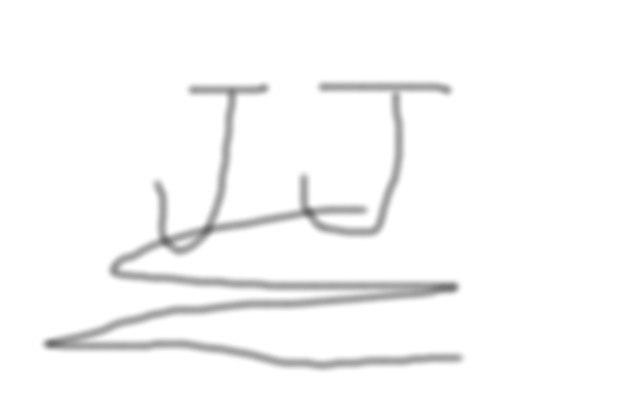
\includegraphics[scale=0.2]{images/firma2}
\end{figure}

\newpage

\tableofcontents

\newpage

\fancypagestyle{miEstilo1}{
   \lhead{1. Introducción}
   %\chead{1. Introducción}
   \rhead{Página \thepage}
   \lfoot{}
   \cfoot{}
   \rfoot{}
}

\pagestyle{miEstilo1}

\section{Introducción}

\subsection{Motivación}

El número de robos y hurtos ha ido creciendo en estos últimos años, y por ello, es necesario la aplicación de medidas preventivas y correctoras que intenten reducir este número.

Hoy en día vivimos en una sociedad informatizada y tecnológica, donde cada uno tiene la capacidad de poder encontrar casi cualquier información allá donde esté, gracias a los dispositivos móviles y a la redes de comunicaciones que usa internet.

¿Quién no lleva un smartphone con conexión de datos en su bolsillo? En España el 85\% de la población hace uso de su smartphone a diario. Estos dispositivos móviles tienen una gran cantidad de usos y aplicaciones, y se han convertido en una herramienta imprescindible en nuestro día a día.

Uniendo tecnología y aplicación de medidas de seguridad basada en videovigilancia, surge la idea de este proyecto; la idea de construir un sistema de videovigilancia de bajo coste que sea fácil de usar, mantener, y lo más importante, que pueda ser controlado desde cualquier parte.

Partiendo de esta idea, se ha investigado y construido una aplicación que cumple con estas expectativas y más, ya que el uso que se le quiera dar puede ir más allá del concepto de videovigilancia para la seguridad. Por ejemplo, se puede utilizar para controlar entradas y salidas en una zona, control parental \ldots, aunque eso sí, dentro de un uso permitido y responsable.

Otro de los principales aspectos de este proyecto, es que su uso no sea de forma privada, es decir, que pueda ser usado por todas las personas que lo deseen. Por este motivo, se ha intentado reducir todo lo posible el coste del hardware, y se ha liberado todo el código fuente, junto con las instrucciones necesarias para la instalación y despliegue de la aplicación.

Toda la información relacionada se puede consultar en el repositorio de Github \cite{ref1}.

\subsection{Objetivos}

El objetivo principal de este proyecto es el de poder construir un sistema de seguridad basado en la videovigilancia, de bajo coste, y accesible a todo el mundo.

\textbf{Objetivos generales}

\vspace{-0.3cm}

\begin{itemize}
	\item Rebajar el coste de los sistemas de videovigilancia habituales.
	\item Alertar a un usuario ante un evento de movimiento generado dentro de una zona controlada.
	\item Almacenar y obtener pruebas (fotos y/o vídeo) tras la detección de cualquier intruso.
	\item Monitorizar y controlar el estado de un entorno.
	\item Aumentar el nivel de seguridad de cualquier tipo de entorno.	
\end{itemize}

\textbf{Objetivos específicos}

\vspace{-0.3cm}

\begin{itemize}
	\item Proporcionar un sistema accesible para todo el mundo y fácil de usar.
	\item Permitir el acceso y gestión del sistema a través de un dispositivo móvil.
	\item Investigar y conocer el uso de los bots de Telegram como medio de interacción entre el usuario y la aplicación back-end desarrollada en este proyecto.
	\item Estudiar el funcionamiento de una Raspberry PI y sus principales componentes para su aplicación en el ámbito del proyecto.
	\item Conocer, diseñar y hacer uso de una arquitectura basada en microservicios que permita el uso de servicios independientes, ágiles y escalables.
	\item Aprender a utilizar mecanismos de aprendizaje automático para poder filtrar y evitar falsos positivos en las alertas generadas.

\end{itemize}

\newpage

\subsection{Estructura del documento}

Este documento está estructurado de la siguiente forma:

\textbf{1. Introducción}: Motivos y objetivos por los cuales se ha desarrollado este proyecto.

\textbf{2. Planificación del proyecto}: Muestra información detallada acerca de las diferentes etapas del proyecto, junto con la planificación prevista.

\textbf{3. Análisis de mercado}: Estudio comparativo acerca de softwares similares al propuesto en este proyecto.

\textbf{4. Tecnologías y herramientas utilizadas}: Breve descripción sobre las tecnologías y herramientas utilizadas para desarrollar este proyecto.

\textbf{5. Descripción de la aplicación: SIVIRA}: Descripción sobre los componentes de la aplicación, la interacción entre ellos, medidas de seguridad aplicadas, interfaz de usuario y descripción de la estructura de archivos y directorios de la aplicación.

\textbf{6. Presupuesto}: Estimación de costes del desarrollo del proyecto junto con una previsión de futuros beneficios en el mercado laboral.

\textbf{7. Conclusiones y trabajos futuros}: Conclusiones tras finalizar el desarrollo del proyecto y posibles mejoras a desarrollar en versiones posteriores.

\textbf{ANEXO}: Información útil sobre la aplicación SIVIRA: guía de instalaciones de componentes, instalación y despliegue de la aplicación y finalmente una guía de usuario.

\newpage



\newpage



\fancypagestyle{miEstilo2}{
   \lhead{2. Planificación}
   %\chead{1. Introducción}
   \rhead{Página \thepage}
   \lfoot{}
   \cfoot{}
   \rfoot{}
}

\pagestyle{miEstilo2}

\section{Planificación}

Como en todo proyecto, realizar una buena planificación es la clave para no fracasar en el desarrollo del proyecto. Por ello, se ha realizado una planificación detallada del proyecto, utilizando el concepto de \textit{iteraciones} y \textit{sprints} para ir distribuyendo el trabajo a lo largo de las semanas, durante las cuales se han ido desarrollando una serie de tareas que cumplen un objetivo específico.

Estos conceptos surgen de los llamados métodos de desarrollo ágiles, en los cuales se intenta descomponer una aplicación o proyecto por funcionalidades, y el objetivo es ir desarrollando y testeando cada una de forma independientes para poder integrarla con el resto.

A continuación se muestra la planificación que se ha previsto para el desarrollo del proyecto.


\subsection{Fase preparatoria}

En esta fase se comenzará el desarrollo del proyecto. Tiene un esfuerzo estimado de X horas. Se realizará un estudio de viabilidad de la idea del proyecto, así como un estudio de mercado, una investigación acerca de las posibles herramientas a usar \ldots.

El objetivo de esta primera fase es tener claro que el proyecto es viable tanto en recursos, tiempo y presupuesto, para que posteriormente comience su desarrollo e implementación.

\large{\textbf{Iteración 1}: Análisis y estudio de la aplicación.}
\hrule

\vspace{0.3cm}

\normalsize

En esta iteración se describirán los principales objetivos de la aplicación, se estudiará sus posibles casos de uso y se elaborará un plan de iteraciones para planificar el desarrollo del proyecto a lo largo del tiempo dispuesto.

Esta iteración se divide en los siguientes sprints:

\textbf{Sprint 1}: Descripción de la aplicación



%\begin{center}
%\begin{tabular}{ | m{5em} | m{1cm}| m{1cm} | } 
%\hline
%cell1 dummy text dummy text dummy text& cell2 & cell3 \\ 
%\hline
%cell1 dummy text dummy text dummy text & cell5 & cell6 \\ 
%\hline
%cell7 & cell8 & cell9 \\ 
%\hline
%\end{tabular}
%\end{center}




\begin{table}[]
\begin{tabular}{|p{4cm}|p{7cm}|p{1.5cm}|p{2.5cm}|}
\hline
\rowcolor[HTML]{000000} 
{\color[HTML]{FFFFFF} Product backlog} & {\color[HTML]{FFFFFF} Descripción}                                  & {\color[HTML]{FFFFFF} Semana} & {\color[HTML]{FFFFFF} T.Previsión} \\ \hline
Objetivos                              & Descripción de los objetivos                                        & 1                             &                                        \\ \hline
Funcionalidades                        & Descripción de las funcionalidades                                  & 1                             &                                        \\ \hline
Motivaciones                           & Motivaciones personales acerca de la temática del proyecto          & 1                             &                                        \\ \hline
Usuarios y escenarios                  & Descripción de los posibles casos de uso de la aplicación propuesta & 1                             &                                        \\ \hline
\end{tabular}
\end{table}






\newpage



\fancypagestyle{miEstilo3}{
   \lhead{3. Análisis de mercado}
   %\chead{1. Introducción}
   \rhead{Página \thepage}
   \lfoot{}
   \cfoot{}
   \rfoot{}
}

\pagestyle{miEstilo3}

\section{Análisis de mercado}

Antes de comenzar con el desarrollo del proyecto, se ha realizado un estudio de mercado para comprobar si hay algún tipo de sistema similar ya implementado, qué características tiene, y qué posibles diferencias habría con el que se tiene pensado implementar.

Es cierto que la raspberry PI tiene infinidades de posibles aplicaciones, y que en la web se puede encontrar todo tipo de tutoriales e ideas para poder explotar al máximo su uso, pero ¿existirá algún tipo sistema de seguridad que sea funcional, fácil de instalar y utilizar?. Para responder a esta pregunta, se ha realizado una búsqueda intensiva en la web y youtube, ya que suelen ser los principales medios donde se publica este tipo de información.

Investigando, se ha descubierto que hay múltiples páginas y vídeos que hacen referencia al uso de una raspberry PI con una cámara, y su posible aplicación para poder visualizar en tiempo real la grabación realizada por la cámara.

A continuación se van a detallar los principales aspectos a destacar de los sistemas encontrados.

\subsection{Proyecto: Build a Raspberry Pi Security Camera Network} \label{sec:pj1}

Este es un proyecto \cite{ref2} que se basa en el uso de una distribución Linux llamada \texttt{motionEyeOS} y de código abierto \cite{ref3} que convierte una raspberry PI en un sistema de videovigilancia.

Si leemos la descripción de este proyecto \cite{ref2}, podemos observar como se hace una pequeña descripción de los componentes necesarios y una guía de instalación del sistema \texttt{motionEyeOS}.

Entre sus principales características, podemos encontrar las siguientes:

\vspace{-0.5cm}

\begin{itemize}
\item \textbf{Acceso restringido}: Consta de unas credenciales (usuario y contraseña) para poder acceder a la visualización y configuración de las cámaras.

\item \textbf{Sistema multicámara}: Es un sistema que soporta la visualización e interacción con múltiples cámaras simultáneamente conectadas en la misma red.

\begin{figure}[h]
	\centering
	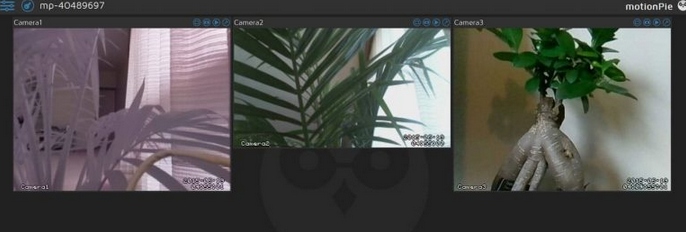
\includegraphics[scale=0.4]{images/1}
	\label{imagen2}
	\caption{Sistema de seguridad con 3 cámaras}
\end{figure}

\item \textbf{Conexión via wifi}: Este sistema soporta la conexión via wifi. Será necesario añadir el SSID y clave de la red.

\item \textbf{Configuración de la cámara}: El sistema consta de un menú para poder configurar la cámara. Los parámetros configurables son:

	\begin{itemize}
	\item Nombre de la cámara: Nombre para poder identificar la cámara.
	\item Filtrado de luz: Filtro para evitar falsos positivos ante el encendido y apagado de una luz.
	\item Brillo automático: Configuración automática de brillo y contraste de luz.
	\item Resolución de la cámara: Configuración para poder modificar la resolución de la cámara.
	\item Rotación de la cámara: Rotación de la imagen de vídeo o cámara.
	\item FPS: Configuración del número de frames por segundo (imágenes por segundo).
	\end{itemize}

\item \textbf{Almacenamiento}: Es posible almacenar los archivos de imagen o vídeo.

\item \textbf{Fecha y hora}: Posibilita la opción de mostrar fecha y hora durente la grabación de un vídeo o la captura de una foto.

\item \textbf{Vídeo streaming}: Permite la visualización del vídeo capturada por las cámaras en tiempo real.

\item \textbf{Detección de movimiento}: El sistema permite la detección de movimiento y en consecuencia la grabación de un vídeo o la captura de una foto.

\item \textbf{Alertas}: Es posible generar alertas via email o webhook cuando se detecta movimiento.

\end{itemize}

\subsection{Proyecto: Raspberry Pi As Low-cost HD Surveillance Camera}\label{sec:pj2}

Este es un proyecto \cite{ref4} bastante simple y centrado en la vigilancia y basado en \texttt{Motion detection software} \cite{ref5}. Este es un software de código abierto y disponible en los repositorios de raspbian para poder monitorizar las señales de vídeo para varios tipos de cámaras (entre ellas la PiCamera).

Algunas de las características de este software son:

\vspace{-0.5cm}

\begin{itemize}
\item Grabación de vídeos y/o capturas de fotos.
\item Visualización de vídeo en tiempo real (streaming).
\item Gestión de actividades y activación de scripts tras dichos eventos.
\item Registro de eventos en bases de datos.
\item Plantillas personalizables para detección de movimiento.
\item Soporte completo de TLS (https) con autenticación y control web para streaming.

\end{itemize}

En este proyecto, se hace una descripción de los componentes necesarios para poder montar este sistema, e incluso se hace una estimación del precio de dichos componentes y se proporciona un enlace de compra.

A continuación se proporciona una guía básica de instalación y configuración, mostrando los siguientes resultados:

\newpage

\begin{figure}[H]
	\centering
	\begin{subfigure}[b]{0.3\textwidth}
		
\includegraphics[width=\textwidth,height=90px]{images/2}
		\caption{Colocación de la cámara}
	\end{subfigure}
	~ 
	\begin{subfigure}[b]{0.3\textwidth}
		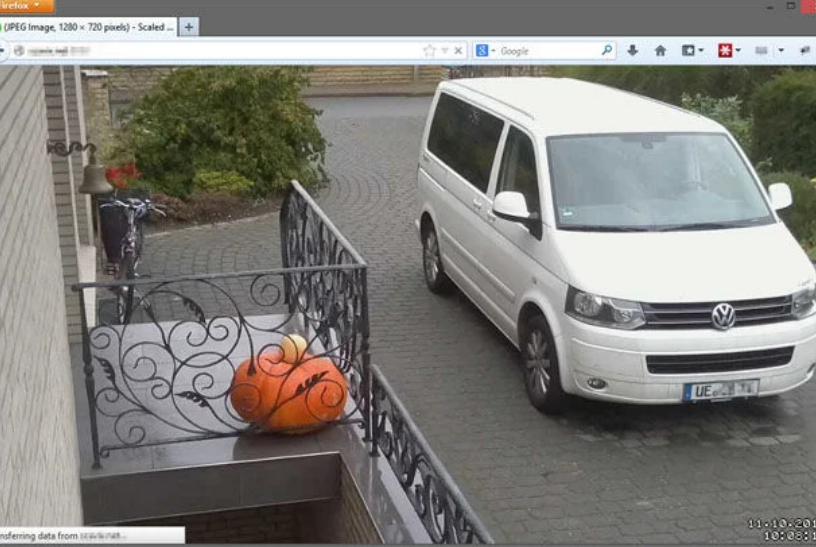
\includegraphics[width=\textwidth,height=90px]{images/3}
		\caption{Streaming}
	\end{subfigure}
	\caption{Sistema de videovigilancia}

\end{figure}

\subsection{Proyecto: sensor de movimiento y cámara con envío de imágenes a correo} \label{sec:pj3}

Este es un proyecto descrito en un vídeo de youtube \cite{ref6} que explica cómo construir un pequeño sistema de seguridad basado en la detección de movimiento, captura de una foto y envío de la foto capturada tras haberse activado la detección de movimiento.

En este vídeo se explica qué componentes son necesarios, cómo conectarlos y se proporciona un script de Python que se encarga de la detección movimiento y envío de la imagen al correo gmail, utilizando librerías de Python como \textit{PiCamera} y \textit{smtplib}.

Este proyecto no tiene complejidad alguna, ya que es muy simple y todo está explicado para cualquier usuario, y es un buen comienzo para empezar a investigar y probar el mundo de la videovigilancia basada en bajo coste.

\subsection{Conclusión}

Investigando por la web, he descubierto que hay muchos tipos de proyectos similares a los mencionados, unos más simples y otros más complejos, pero en general todos comparten el objetivo de poder vigilar una zona a través de una cámara y una raspberry PI.

\newpage

Otro de los principales aspectos a destacar, es que la mayoría hacen el uso del software libre \texttt{motionEyeOS} o \texttt{motion agent detection} que se han mencionado en las secciones \ref{sec:pj1} y \ref{sec:pj2}.

El objetivo de este proyecto no es 'volver a reinventar la rueda` sino hacer de este un proyecto innovador y con un valor añadido respecto al resto.

Por ello, se ha diseñado y propuesto un sistema que cumpla con la mayoría de características de proyectos similares, combinando lo mejor de cada uno, y añadiendo nuevas funcionalidades adicionales que hagan que sea una de las mejores opciones a la hora de plantearse implementar un sistema de videovigilancia de bajo coste.

Según he podido observar, hay muchos proyectos en los que la documentación es escasa y no muy concisa, además de realizar instalaciones y configuraciones a bajo nivel. Esto hace que cualquier usuario no tenga acceso a este tipo de aplicaciones, ya que requieren un usuario medio-avanzado en conocimientos informáticos.

Por ello, se ha tenido en cuenta la simplicidad del software y su fácil gestión y uso, además de intentar cubrir todos los principales aspectos de una videovigilancia.

En las siguientes secciones, se mostrará más en detalle qué funcionalidades tiene esta aplicación, pero para mostrar sus principales aspectos clave y diferenciadores respecto al resto se va a realizar una comparación, tal y como se puede observar en la siguiente tabla.


Observando la tabla \ref{table:1}, se puede comprobar como la aplicación propuesta cumple con la mayoría de las características del resto de proyectos actuales, y mejora en otros aspectos.

Como aspecto a destacar, decir que el proyecto propuesto consta de una aplicación backend y una aplicación multiplataforma de usuario, además de ser fácil de usar y estar documentada. Estos aspectos principales aportan una gran versatilidad a este proyecto, siendo sin duda la mejor opción hasta el momento desarrollada en el ámbito de la videovigilancia de raspberry PI.

También, como trabajos futuros, se desea implementar la funcionalidad multicámara, haciendo posible la interacción con más de una cámara simultáneamente.

\newpage

\begin{table}[h!]
\centering
\begin{tabular}{|l|c|c|c|c|}
\hline
\rowcolor[HTML]{EFEFEF} 
 \textbf{ Proyectos} & \hyperref[sec:pj1]{Proyecto 1}  & \hyperref[sec:pj2]{Proyecto 2} & \hyperref[sec:pj3]{Proyecto 3} & Mi propuesta \\ \hline
Captura de imagen & \cmark & \cmark  & \cmark & \cmark \\ \hline
\rowcolor[HTML]{fcfcfc} 
Grabación de vídeo & \cmark  & \cmark  & \xmark & \cmark \\ \hline
Streaming & \cmark  & \cmark & \xmark & \cmark \\ \hline
\rowcolor[HTML]{fcfcfc} 
Alertas & \cmark  & \cmark & \cmark & \cmark \\ \hline
Filtrado de alertas inteligente & \xmark   & \xmark & \xmark & \cmark \\ \hline
\rowcolor[HTML]{fcfcfc} 
Aplicación de usuario & \xmark & \xmark & \xmark & \cmark \\ \hline
Soporte multicámara & \cmark  & \cmark & \xmark & \xmark \\ \hline
\rowcolor[HTML]{fcfcfc} 
Fácil instalación y uso & \xmark  & \xmark & \cmark & \cmark \\ \hline
Cámara configurable & \cmark  & \xmark & \xmark & \cmark \\ \hline
\rowcolor[HTML]{fcfcfc} 
Documentación & \xmark & \xmark & \xmark & \cmark \\ \hline
Almacenamiento de eventos & \xmark  & \cmark & \xmark & \cmark \\ \hline
\end{tabular}
\caption{Comparativa de los distintos proyecto}
\label{table:1}
\end{table}

\color{black}


\newpage



\fancypagestyle{miEstilo4}{
   \lhead{4. Tecnologías y herramientas usadas}
   %\chead{1. Introducción}
   \rhead{Página \thepage}
   \lfoot{}
   \cfoot{}
   \rfoot{}
}

\pagestyle{miEstilo4}

\section{Tecnologías y herramientas utilizadas}

Para el desarrollo de este proyecto se han utilizado una gran cantidad de herramientas y tecnologías de código abierto. A continuación se muestra cada una de ellas.

\subsection{Diseño}

Para el diseño de este proyecto, se han realizado prototipos y diagramas para poder diseñar la arquitectura y principales componentes de la aplicación, además de la interacción de los componentes con el resto. Para realizar esto, se ha utilizado el siguiente software:

\textbf{Draw.io}

Draw.io \cite{ref7} es una aplicación para diseño y diagramas de aplicaciones. Es un servicio gratis de Google y de código abierto.

Este software se ha utilizado para diagramas de diseño de interfaz.

\begin{figure}[h]
	\centering
	
\includegraphics[scale=0.5]{images/4}
\end{figure}

\textbf{Visual paradigm} 

Visual paradigm \cite{ref8}  es un software de modelado UML que nos permite analizar, diseñar,
codificar, probar y desplegar. Dibuja todo tipo de diagramas UML, genera código fuente a
partir de dichos diagramas y también posibilita la elaboración de documentos.


\begin{figure}[h]
	\centering
	
\includegraphics[scale=0.5]{images/5}
\end{figure}

Este software se ha utilizado para la generación del diagrama de clases e interacción entre componentes.

\newpage

\subsection{Sistema control de versiones}

Los sistemas de control de versiones \cite{ref9} son programas que tienen como objetivo controlar los cambios en el desarrollo de cualquier tipo de software, permitiendo conocer el estado actual de un proyecto, los cambios que se le han realizado a cualquiera de sus piezas, las personas que intervinieron en ellos \ldots

El control de versiones es una de las tareas fundamentales para la administración de un proyecto de desarrollo de software en general. Surge de la necesidad de mantener y llevar control del código que vamos programando, conservando sus distintos estados. Es absolutamente necesario para el trabajo en equipo, pero resulta útil incluso a desarrolladores independientes. 

Por este motivo, no he dudado en utilizar un sistema de control de versiones. El sistema de control de versiones me ha facilitado mucho la gestión y seguimiento del proyecto. El sitema que he utilizado ha sido \texttt{git}, y como medio de alojamiento para este proyecto he utilizado  \texttt{Github}.

\textbf{Git}

\texttt{Git} \cite{ref10}  es un sistema de control de versiones distribuido, de código libre y multiplataforma que permite la gestión de repositorios software a través de una línea de comandos \cite{ref9}.

Para este proyecto, se ha creado un repositorio donde se ha almacenado todo el código fuente de la aplicación junto con sus cambios a lo largo de su desarrollo.

\begin{figure}[h]
	\centering
	
\includegraphics[scale=0.25]{images/6}
\end{figure}

\textbf{Github}

\texttt{Github} \cite{ref11} es un servicio para alojamiento de repositorios de software gestionados por el sistema de control de versiones \texttt{Git}. En definitiva, \texttt{Github} es un sitio web pensado para hacer posible el compartir el código de una manera más fácil y al mismo tiempo darle popularidad a la herramienta de control de versiones en sí, que es \texttt{Git}.

Este proyecto se ha ido alojando en el repositorio de Github \url{https://github.com/jmv74211/TFM_security_system_PI}.

\begin{figure}[h]
	\centering
	
\includegraphics[scale=0.2]{images/7}
\end{figure}

\subsection{Lenguajes de programación y lenguajes de marcas}

La implementación de este proyecto está desarrollada básicamente en \texttt{Python}. También se ha hecho uso de otros lenguajes de programación para alguna tarea en particular.

A continuación se muestran los lenguajes de programación utilizados.

\textbf{Python}

\texttt{Python} es un lenguaje de programación interpretado, de alto nivel y de propósito general. Este lenguaje de programación viene instalado predeterminadamente en casi todos los sistemas operativos, y consta de un gran número de bibliotecas para realizar una gran cantidad de tareas.

\texttt{Python} se ha utilizado como lenguaje de programación base, con aproximadamente un 90\% del código fuente total. Básicamente he elegido este lenguaje ya que Raspberry PI posee bibliotecas para interaccionar con \texttt{Python}, y con el resto de componentes involucrados.

\begin{figure}[h]
	\centering
	
\includegraphics[scale=0.13]{images/8}
\end{figure}

\textbf{HTML, CSS y Javascript}

Para poder visualizar el streaming de vídeo a través del navegador, ha sido necesario implementar una pequeña página web utilizando \texttt{HTML} y \texttt{CSS}. Respecto a la parte de conexión entre la cámara y el navegador se ha utilizado \texttt{Python} para crear el servidor HTTP y la conexión websocket, y una biblioteca de funciones de \texttt{Javascript} para la transmisión de datos.

\vspace{-0.5cm}

\begin{figure}[h]
	\centering
	
\includegraphics[scale=0.7]{images/9}
\end{figure}

\vspace{-1cm}

\textbf{BASH}

Bash es un intérprete de comandos que ejecuta, una por una, las instrucciones introducidas por el usuario o contenidas en un script y devuelve los resultados. En otras palabras, actúa como interfaz entre el kernel Linux y los usuarios o programas del modo texto. Además, incorpora numerosas utilidades de programación y mejoras sobre sh, su shell predecesora. Debido a que es una herramienta desarrollada por GNU, suele ser utilizada por defecto en las distros actuales.

\begin{figure}[h]
	\centering
	
\includegraphics[scale=0.15]{images/10}
\end{figure}

En este proyecto se ha programado un script en \texttt{bash} para iniciar o parar la aplicación.

\subsection{Bibliotecas y frameworks externos}

Para la implementación de este proyecto, se han utilizado un gran número de bibliotecas para poder interaccionar entre sus distintos componentes.

A continuación se describen brevemente las bibliotecas y frameworks utilizados.

\newpage

\textbf{PiCamera}

\texttt{PiCamera} \cite{ref12} es una biblioteca de \texttt{Python} que proporciona una gran cantidad de funciones para interaccionar directamente con la cámara de la Raspberry PI.

Esta biblioteca ha sido utilizada en los módulos que interactúan directamente con el recurso hardware de la cámara.


\begin{figure}[h]
	\centering
	
\includegraphics[scale=0.09]{images/11}
\end{figure}

\textbf{pyTelegramBotAPI}

\texttt{pyTelegramBotAPI} \cite{ref13} es una biblioteca de funciones de alto nivel que hace uso de la API de Telegram.

En este proyecto se ha utilizado para crear el bot de Telegram, que será la aplicación con la que el usuario interaccionará, y éste a su vez con la API desarrollada en la aplicación backend.

\begin{figure}[h]
	\centering
	
\includegraphics[scale=0.22]{images/12}
\end{figure}

\textbf{Flask}

\texttt{Flask} \cite{ref14} es un framework ligero de aplicaciones web WSGI. Está diseñado para hacer que el despliegue de una aplicación sea rápida y fácil, con la capacidad de escalar a aplicaciones complejas.

En este proyecto se ha utilizado para implementar varios servicios web, como la API principal que interactúa con el resto de módulos y componentes.

\begin{figure}[h]
	\centering
	
\includegraphics[scale=0.19]{images/13}
\end{figure}

\textbf{Celery}

\texttt{Celery} \cite{ref15} es una implementación de una cola de tareas para aplicaciones web de \texttt{Python} que se utiliza para ejecutar tareas de forma asíncrona.

En este proyecto se ha utilizado principalmente en la API y en el agente de movimiento. El objetivo es poder realizar peticiones, y que la API atienda al mayor número de ellas, devolviendo la respuesta tras la ejecución de las tareas, sin producir ningún tipo de espera entre las comunicaciones (Más información en la sección \ref{sec:composer}).

\vspace{-0.6cm}

\begin{figure}[h]
	\centering
	
\includegraphics[scale=0.15]{images/14}
\end{figure}

\vspace{-1.4cm}

\textbf{RPi.GPIO}

\texttt{RPi.GPIO} \cite{ref16} es un paquete que provee de una clase para controlar las conexiones GPIO de la Raspberry PI.

En este proyecto es usado para recibir la señal del sensor de movimiento, de forma que es posible saber cuándo se ha activado.

\begin{figure}[h]
	\centering
	
\includegraphics[scale=0.15]{images/15}
\end{figure}

\vspace{-0.6cm}

\textbf{Tensorflow}

\texttt{Tensorflow}  es una plataforma de código abierto para aprendizaje automático. Cuenta con un ecosistema completo y flexible de herramientas, bibliotecas y recursos que permiten a los investigadores impulsar el estado del arte en machine learning y a los desarrolladores construir y desplegar fácilmente aplicaciones potenciadas por el machine learning.

En este proyecto se ha utilizado para construir un agente que sea capaz de reconocer objetos en una foto utilizando un modelo ligero preentrenado (más información en la sección \ref{sec:composer}).

\begin{figure}[h]
	\centering
	
\includegraphics[scale=0.12]{images/19}
\end{figure}

\textbf{Requests}

\texttt{Requests} \cite{ref18} es una librería HTTP con licencia Apache2, escrita en \texttt{Python}. Permite enviar peticiones HTTP/1.1, además de añadir cabeceras, datos de formulario, archivos y parámetros con diccionarios \texttt{Python} simples, y acceder a los datos de respuesta de la misma manera.

En este proyecto ha sido utilizado para la comunicación entre los servicios a través de sus API's.

\begin{figure}[h]
	\centering
	
\includegraphics[scale=0.08]{images/20}
\end{figure}

\vspace{-0.5cm}

\subsection{Documentación}

\textbf{LaTeX}

Para elaborar la documentación se ha utilizado \texttt{LaTeX} \cite{ref19} que es un sistema de elaboración de documentos para una composición tipográfica de alta calidad. Se utiliza con mayor frecuencia para documentos técnicos o científicos de mediano a gran tamaño, pero se puede utilizar para casi cualquier forma de publicación.

Para este proyecto se ha utilizado \texttt{LaTeX}, utilizando la distribución \texttt{TEXLive} \cite{ref20} que proporciona un sistema TeX completo con binarios para la mayoría de las versiones de Unix, incluyendo GNU/Linux, macOS, y también Windows. Incluye todos los principales programas relacionados con TeX, paquetes de macros y fuentes que son software libre, incluyendo soporte para muchos idiomas en todo el mundo. 

\begin{figure}[h]
	\centering
	
\includegraphics[scale=0.18]{images/16}
\end{figure}

\textbf{TeXstudio}

\texttt{TeXstudio} \cite{ref21} es un entorno integrado para crear documentos LaTeX. El objetivo es conseguir que escribir LaTeX sea lo más fácil y cómodo posible.

Para este proyecto se ha utilizado la versión \textit{2.12.14}.

\begin{figure}[h]
	\centering
	
\includegraphics[scale=0.3]{images/17}
\end{figure}

\subsection{Entorno de desarrollo}

El entorno de desarrollo ha sido un aspecto muy importante para la implementación del proyecto, ya que el código se está ejecutando en una Raspberry PI que tiene recursos muy limitados, y los editores o entornos que puede utilizar no son los más cómodos.

Por este motivo, he estado investigando si se puede realizar un desarrollo de la aplicación vía remota. Leyendo foros, observé que el entorno de desarrollo \texttt{pycharm} tiene la opción de poder crear y desarrollar un proyecto vía SSH.

\textbf{Pycharm}

Pycharm \cite{ref22} es un entorno de desarrollo profesional de \texttt{Python}. Gracias a dicho entorno de desarrollo he podido gestionar el proyecto de forma local, ya que los cambios generados se han sincronizado y ejecutado en la Raspberry PI a través de SSH.

En este proyecto se ha utilizado la versión \textit{2019.1.3 Profesional edition}, licencia académica que he obtenido gracias a la UGR. 

\begin{figure}[h]
	\centering
	
\includegraphics[scale=0.06]{images/18}
\end{figure}


\subsection{Otros servicios}

\textbf{Rabbit MQ} 

\texttt{RabbitMQ} \cite{ref23} es un broker de mensajes que acepta y reenvía mensajes. Un broker de mensajes actúa como plataforma intermediaria a la hora de procesar la comunicación entre dos aplicaciones.

En este proyecto ha sido utilizado para crear dos colas de procesos, utilizados por las tareas asíncronas desarrolladas con \texttt{celery}.

\begin{figure}[h]
	\centering
	
\includegraphics[scale=0.2]{images/21}
\end{figure}

\textbf{Telegram bot API} 

Los bots de Telegram \cite{ref24} son aplicaciones de terceros que se ejecutan dentro de Telegram. Los usuarios pueden interactuar con los bots enviándoles mensajes, comandos y peticiones. Se pueden controlar estos bots usando peticiones HTTPS a la API de bot de Telegram.

En este proyecto se ha utilizado para crear un bot de Telegram que interactúe con el usuario y con la aplicación backend desarrollada.

\begin{figure}[h]
	\centering
	
\includegraphics[scale=0.1]{images/22}
\end{figure}




\newpage



\fancypagestyle{miEstilo5}{
   \lhead{5. Descripción de la aplicación}
   %\chead{1. Introducción}
   \rhead{Página \thepage}
   \lfoot{}
   \cfoot{}
   \rfoot{}
}

\pagestyle{miEstilo5}

\section{Descripción de la aplicación: SIVIRA}

El sistema de videovigilancia con una Raspberry PI (\texttt{SIVIRA}) es una aplicación que nos permite construir un sistema de seguridad basado en la videovigilancia de bajo coste utilizando una Raspberry PI , una cámara y un sensor de movimiento.

La idea es poder controlar el sistema a través de una aplicación móvil, con la que el usuario pueda conectarse desde cualquier parte y tener acceso a su información y sistema de seguridad. Las funciones principales de este sistema son las siguientes:

\begin{itemize}
\item \textbf{Sistema automático} de alertas generadas al capturar el movimiento.
\item \textbf{Sistema manual} para grabar vídeo o capturar una foto instantáneamente.   
\item \textbf{Sistema de streaming} para visualizar la imagen en tiempo real.
\end{itemize}

Además, podemos realizar configuraciones personalizadas a la cámara, como por ejemplo, cambiar la resolución, rotación... y la opción de poder activar un agente que filtre las alertas automáticas, generando únicamente alertas cuando se detecta a una persona en una imagen (evitar falsos positivos).



\fancypagestyle{miEstilo501}{
   \lhead{5.1 Arquitectura de la aplicación}
   \rhead{Página \thepage}
   \lfoot{}
   \cfoot{}
   \rfoot{}
}

\pagestyle{miEstilo501}


\subsection{Arquitectura de la aplicación}

Esta aplicación consta de una \textbf{arquitectura basada en microservicios}. Una arquitectura de microservicios \cite{ref25} consta de una colección de servicios autónomos y pequeños. Los servicios son independientes entre sí y cada uno debe implementar una funcionalidad de negocio individual.

En cierto modo, los microservicios son la evolución natural de las arquitecturas orientadas a servicios aunque con ciertas diferencias.

\newpage

\textbf{¿Por qué se ha utilizado esta arquitectura?}

En primer lugar, se ha realizado una descomposición de los principales componentes necesarios para construir la aplicación, y se ha observado que hay funcionalidades independientes que se pueden comunicar entre sí para integrarse en la aplicación. Esto aporta una gran serie de ventajas respecto a un diseño monolítico \cite{ref26} como las siguientes:

\begin{itemize}
\item \textbf{Implementaciones independientes}: Es posible actualizar un servicio sin volver a implementar toda la aplicación y revertir o poner al día una actualización si algo va mal. Las correcciones de errores y las publicaciones de características son más fáciles de administrar y entrañan menos riesgo, por lo tanto, facilitan el mantenimiento de este software.

\item \textbf{Desarrollo independiente}: Cada microservicio se ha ido desarrollando a lo largo de una iteración y de forma independiente al resto. Esto ha agilizado bastante la tarea, ya que las modificaciones y errores no se retropropagaban.

\item \textbf{Fácil escalabilidad}: Cada microservicio puede ser escalado de forma independiente al resto. Por ejemplo, en el caso de que sea necesario escalar la detección de objetos en imágenes, bastaría con replicar el microservicio de detección de objetos y balancear las peticiones entre ellos.

\item \textbf{Fácil integración y alta cohesión}: Un sistema de microservicios se puede integrar y adaptar a casi cualquier sistema. Por ejemplo, en el caso de que quisiera añadir un sistema multicámara a la aplicación, bastaría con añadir una nueva capa superior de abstracción sobre el software desarrollado y se integraría perfectamente.
\end{itemize}

Basándome en esta arquitectura basada en microservicios, se ha diseñado el siguiente sistema (ver figura \ref{img:arquitectura}).

\newpage

\begin{figure}[h]
	\centering
	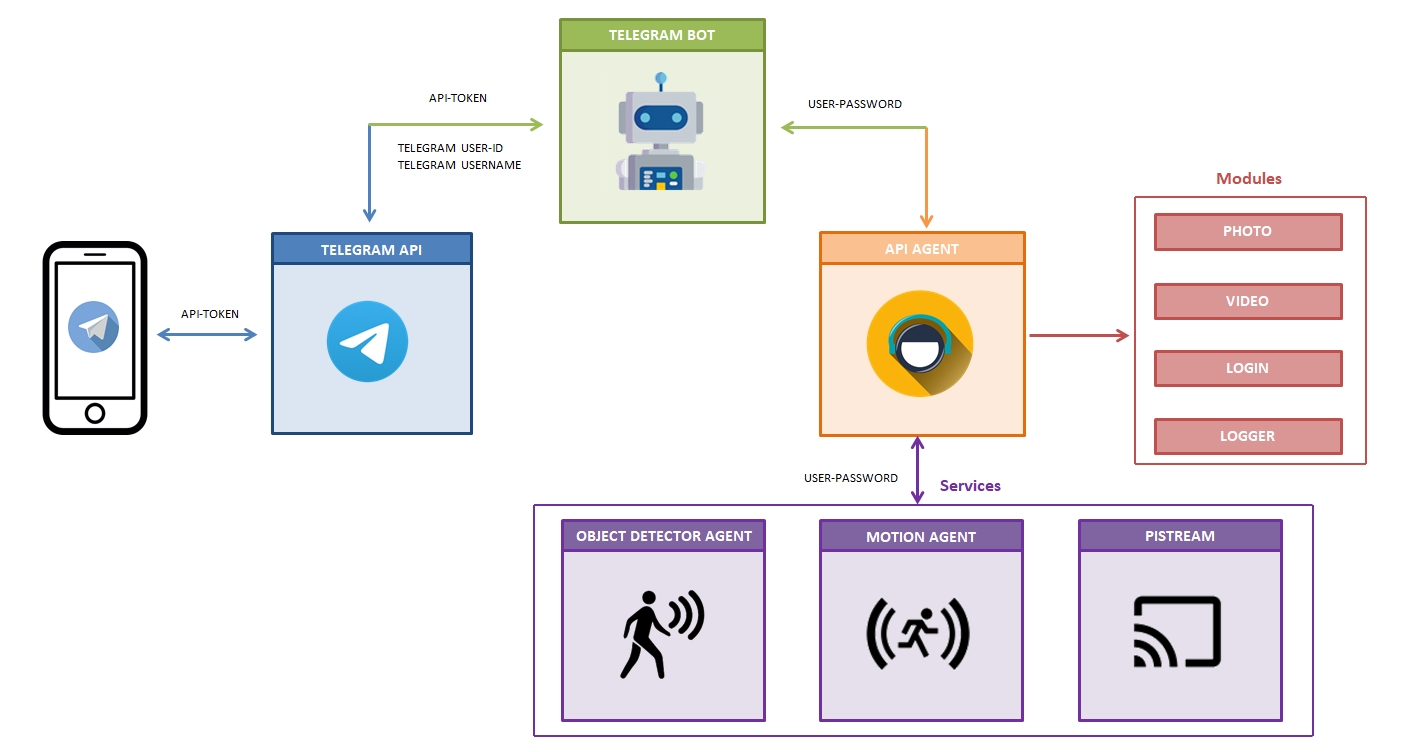
\includegraphics[scale=0.4]{images/23}
	\caption{Arquitectura de la aplicación}
	\label{img:arquitectura}
\end{figure}

En primer lugar tenemos los \textbf{módulos} de la aplicación (ver figura \ref{img:modulos}) que implementan un conjunto de funcionalidades para comunicarse con el módulo hardware de la cámara de la Raspberry PI, autenticación y logs.

\begin{figure}[h]
	\centering
	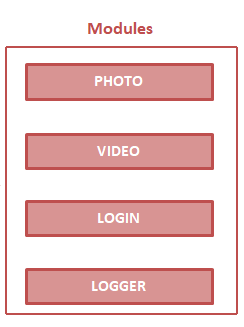
\includegraphics[scale=0.4]{images/24}
	\caption{Módulos de la aplicación}
	\label{img:modulos}
\end{figure}

A continuación tenemos el \textbf{API agent} (ver figura \ref{img:api}). Este es un servicio web que inicia la API que conecta con el resto de módulos de la aplicación.

\begin{figure}[h]
	\centering
	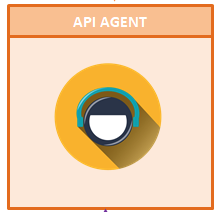
\includegraphics[scale=0.35]{images/25}
	\caption{API agent}
	\label{img:api}
\end{figure}

\newpage

Esta API importa y hace uso de los módulos de la aplicación. 

\begin{figure}[h]
	\centering
	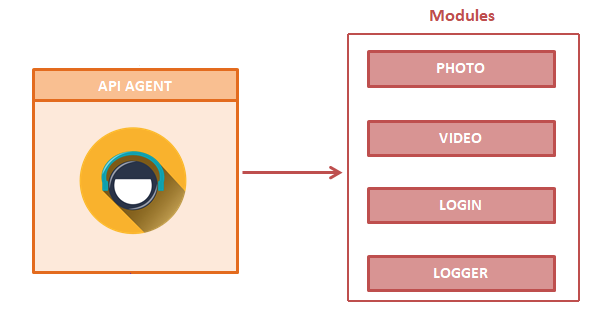
\includegraphics[scale=0.35]{images/27}
	\caption{Conexión entre la API y los módulos}
	\label{img:conexionapimodulos}
\end{figure}

Por otra parte, tenemos un conjunto de servicios que se inician de forma independiente y proporcionan las funcionalidades de detección de objetos en imágenes, detección de movimiento y servicio de streaming.

\begin{figure}[h]
	\centering
	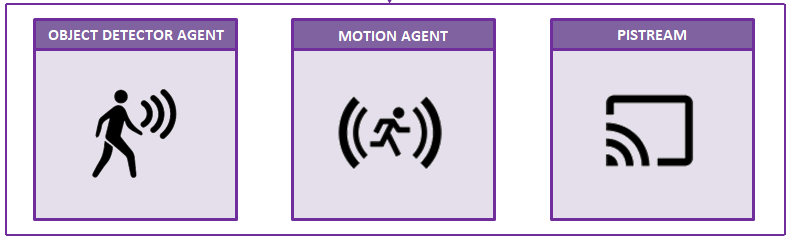
\includegraphics[scale=0.35]{images/26}
	\caption{Servicios de la aplicación}
	\label{img:serviciosaplicacion}
\end{figure}

La API está conectada con todo este conjunto de servicios y tiene la capacidad de poder gestionarlos.

\begin{figure}[h]
	\centering
	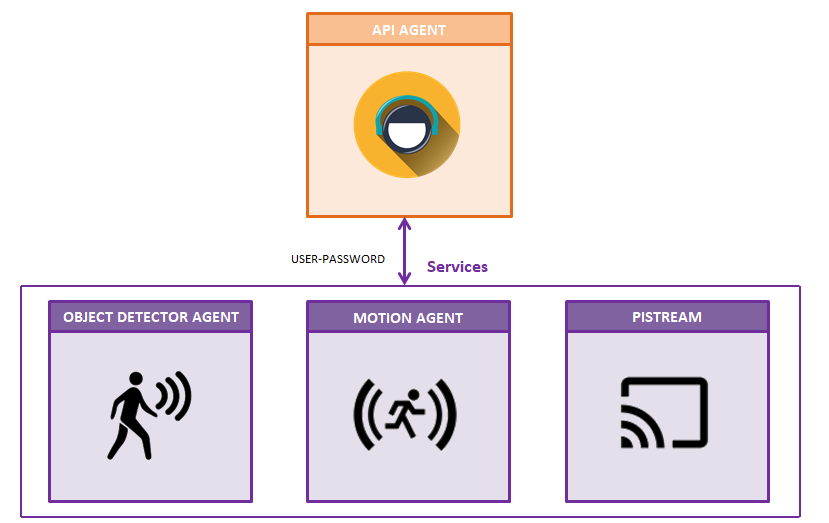
\includegraphics[scale=0.35]{images/28}
	\caption{Conexión entre los servicios y la API}
	\label{img:conexionserviciosapi}
\end{figure}

En la figura \ref{img:conexionmodulosserviciosapi} podemos ver, como quedan unidos todos estos componentes entre sí.

\newpage


\begin{figure}[h]
	\centering
	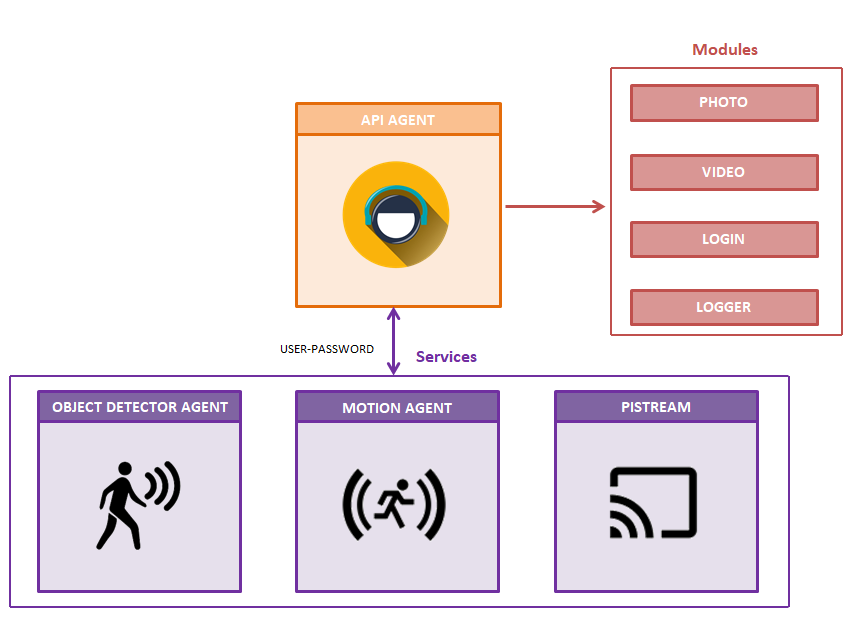
\includegraphics[scale=0.35]{images/35}
	\caption{Conexión de módulos y servicios con la API}
	\label{img:conexionmodulosserviciosapi}
\end{figure}

El siguiente componente es el \textbf{bot de Telegram}. Este bot es un proceso que se ejecuta junto a la API, cuyo objetivo es conectar la API de Telegram con la API de la aplicación.

\begin{figure}[h]
	\centering
	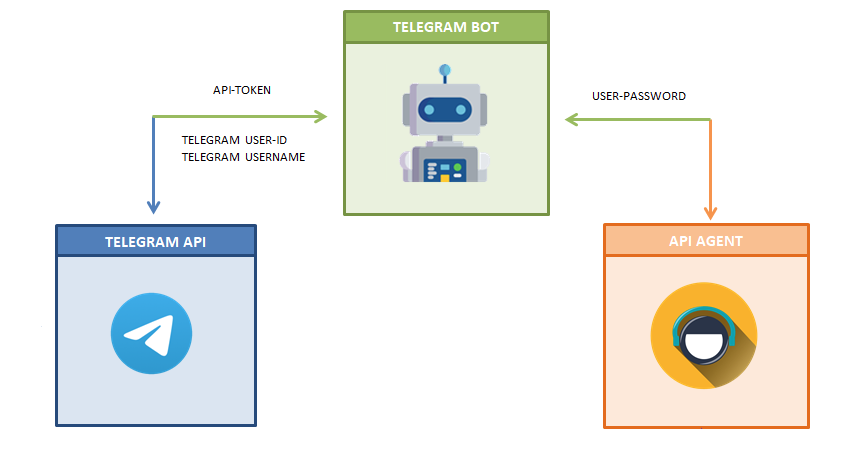
\includegraphics[scale=0.35]{images/34}
	\caption{Conexión entre el bot de Telegram y la API}
	\label{img:conexionbotapitelegram}
\end{figure}

Finalmente, el usuario puede interactuar con la aplicación (\texttt{SIVIRA}), haciendo uso de la aplicación multiplataforma \texttt{Telegram}, usando el bot que se ha creado.

\begin{figure}[h]
	\centering
	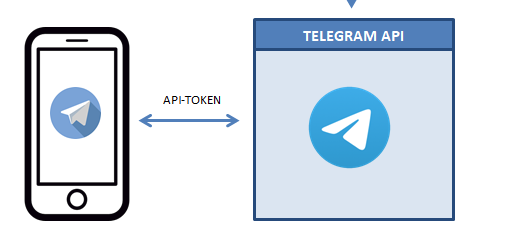
\includegraphics[scale=0.35]{images/33}
	\caption{Conexión entre el usuario y la aplicación}
	\label{img:usuariotelegram}
\end{figure}

\newpage




\fancypagestyle{miEstilo502}{
   \lhead{5.2 Descripción de los componentes y servicios}
   \rhead{Página \thepage}
   \lfoot{}
   \cfoot{}
   \rfoot{}
}

\pagestyle{miEstilo502}


\subsection{Descripción de los componentes y servicios} \label{sec:composer}

La aplicación (SIVIRA) desarrollada en este proyecto está compuesta por los siguientes componentes:

\subsubsection{Módulos}

Los módulos son un conjunto de funciones cuyo objetivo es encapsular funcionalidades que después serán utilizadas por el resto de componentes de la aplicación (ver figura \ref{img:modulos}). A continuación se realiza una descripción de cada uno de ellos.

\textbf{Logger}

Módulo cuyo objetivo es poder capturar y almacenar los logs de la aplicación en ficheros independientes para monitorizar el estado de la aplicación. Su implementación parte de una clase abstracta base, cuyo objetivo es definir las propiedades y métodos que tendrán todas las clases que implementarán los logs del sistema. 

\begin{figure}[h]
	\centering
	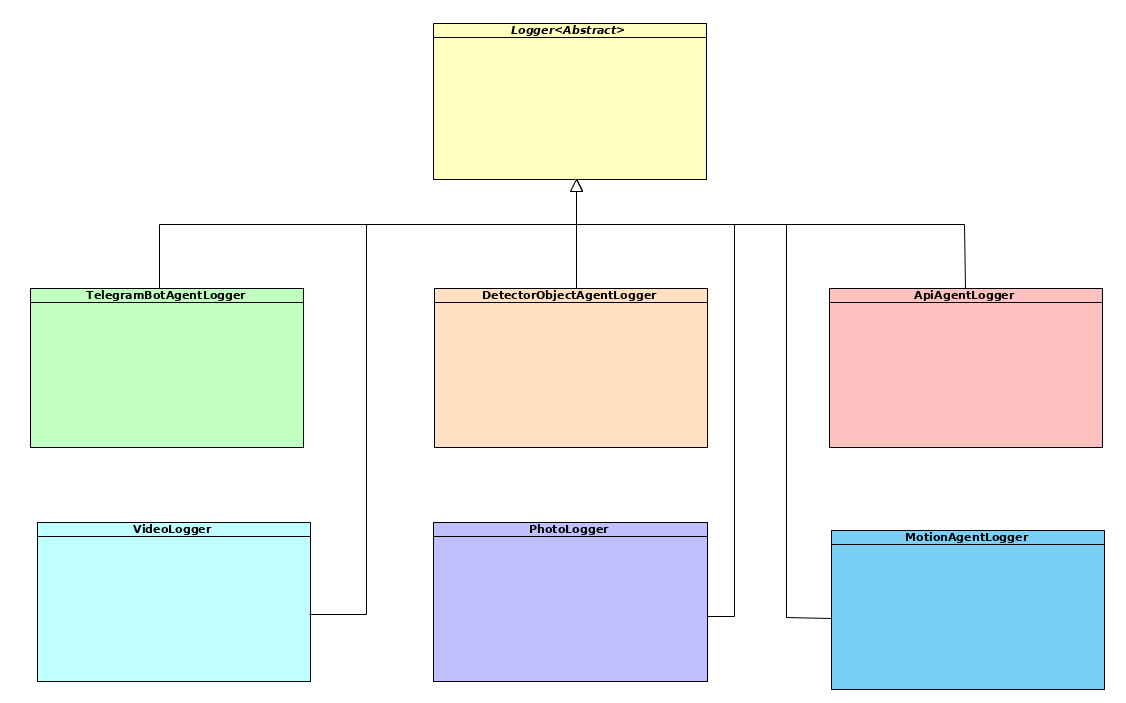
\includegraphics[scale=0.45]{images/83}
	\caption{Relación de herencia entre las clases logger}
\end{figure}

\newpage

Por defecto, los logs son mostrados y almacenados de la siguiente forma:

\begin{itemize}
\item \textbf{Consola}: Corresponde a la salida \texttt{stdout}. Todo los logs por encima de un nivel determinado de prioridad será mostrado por la salida de consola.

\item \textbf{Archivo de módulo}: Cada módulo y microservicio tendrán un fichero de log independiente para poder monitorizar su comportamiento a lo largo de su ejecución.

\item \textbf{Archivo de la aplicación}: La aplicación consta de un archivo de logs donde se almacenan todos los logs de módulos y microservicios de forma conjunta.

\item \textbf{Archivo de errores}: Todos los errores que surjan en cualquier módulo o microservicio son almacenados en este fichero para poder comprobar el estado de la aplicación.

\end{itemize}

Los niveles de logs que se han establecido son los siguientes:

\begin{itemize}

\item \textbf{DEBUG}: Nivel destinado a la depuración del código. Este nivel solo genera log en la salida por pantalla, y no se almacena en ningún fichero.

\item \textbf{INFO}: Nivel destinado a mostrar un mensaje informativo sobre alguna acción llevada a cabo. Estos logs son almacenados en el fichero de módulo correspondiente, en el fichero de logs de la aplicación y mostrados por pantalla.

\item \textbf{WARNING}: Nivel destinado a mostrar un mensajes de advertencia por posible mal uso de las llamadas a funciones, o simplemente porque algunas de ellas están '{deprecated}`. Estos logs son almacenados en el fichero de módulo correspondiente, en el fichero de logs de la aplicación y mostrados por pantalla.

\item \textbf{ERROR}: Nivel destinado a mostrar mensajes de error, que no son críticos para el sistema, y por lo tanto la aplicación sigue ejecutándose a pesar de producirse dichos errores. Estos logs son almacenados en el fichero de módulo correspondiente, en el fichero de logs de la aplicación, en el fichero de errores de la aplicación.

\item \textbf{CRITICAL}: Nivel destinado a mostrar mensajes de errores críticos que provocan el fallo de la aplicación. Estos logs son almacenados en el fichero de módulo correspondiente, en el fichero de logs de la aplicación, en el fichero de errores de la aplicación.

\end{itemize}



El formato por defecto de los logs es el siguiente:

\begin{itemize}
\item \textbf{Formato del archivo de errores}: \texttt{[Nivel:FechaHora:NombreArchivo:Función:Línea] Mensaje}. Por ejemplo:

\vspace{-1cm}

\begin{verbatim}

[ERROR:2019-08-15 13:10:11,597:logger.py:error:112x = set] Error while
trying to send an alert to Detector API agent with address 
http://192.168.1.100:11000.¿It is running?

\end{verbatim}


\vspace{-1cm}

\item \textbf{Formato del resto de logs}: \texttt{[Nivel:FechaHora] Mensaje}. Por ejemplo:

\vspace{-1.2cm}

\begin{verbatim}

[INFO:2019-08-13 18:35:03,278] A 5 seconds video is being 

\end{verbatim}

\end{itemize}

\vspace{-1.2cm}

Todos los ficheros de logs son almacenados en el directorio llamado \texttt{logs}. Dentro de dicho directorio, nos encontraremos los siguientes ficheros de logs:

\vspace{-0.4cm}

\begin{itemize}
\item \textbf{API\_agent.log}: Logs correspondientes a la API.
\item \textbf{detector\_object\_agent.log}: Logs correspondientes al agente detector de objetos.
\item \textbf{photo\_module.log}: Logs correspondientes al módulo de fotos.
\item \textbf{video\_module.log}: Logs correspondientes al módulo de vídeo.
\item \textbf{motion\_agent.log}: Logs correspondientes al agente detector de movimiento.
\item \textbf{security\_system\_PI\_app\_ERROR.log}: Logs correspondientes a los errores obtenidos por cualquier módulo o microservicio.
\item \textbf{security\_system\_PI\_app.log}: Logs correspondientes a los generados por módulos y microservicios a lo largo de su ejecución.
\item \textbf{telegram\_bot\_agent.log}: Logs correspondientes al bot de Telegram.

\end{itemize}

La implementación de este módulo puede comprobarse en este \href{https://github.com/jmv74211/TFM_security_system_PI/blob/master/src/modules/logger.py}{enlace}.

\textbf{Photo} 

Módulo que implementa la clase \texttt{Photo} con la que se pretende administrar el recurso de la cámara de la Raspberry PI para capturar fotografías, además de establecer los diferentes parámetros de la cámara como resolución, rotación \ldots

Esta clase añade una capa de abstracción a la biblioteca \texttt{PiCamera} \cite{ref12}, para permitir conectarse con el recurso de la cámara de forma personalizada.

Las funcionalidades que aporta este módulo son las siguientes:

\vspace{-0.5cm}

\begin{itemize}
\item Capturar una fotografía.
\item Realizar una captura secuencial de fotografías en un intervalo de tiempo
\item Establecer la configuración de la cámara: Rotación, resolución, giro horizontal o giro vertical.

\end{itemize}

\vspace{-0.5cm}

La implementación de este módulo puede comprobarse en este \href{https://github.com/jmv74211/TFM_security_system_PI/blob/master/src/modules/photo.py}{enlace}.

\textbf{Video} 

Módulo que implementa la clase \texttt{Video} con la que se pretende administrar el recurso de la cámara de la Raspberry PI para realizar grabaciones de vídeo, además de establecer los diferentes parámetros de la cámara como resolución, rotación \ldots

Esta clase añade una capa de abstracción a la biblioteca \texttt{PiCamera} \cite{ref12}, para permitir conectarse con el recurso de la cámara de vídeo de forma personalizada.

Las funcionalidades que aporta este módulo son las siguientes:

\vspace{-0.5cm}

\begin{itemize}
\item Realizar una grabación de vídeo.
\item Conversión de formato de vídeo \texttt{.h264} a \texttt{.mp4} (compatible con telegram).
\item Establecer la configuración: Rotación, resolución, giro horizontal, giro vertical y mostrar hora y fecha durante la grabación de vídeo. .

\end{itemize}

\vspace{-0.5cm}

La implementación de este módulo puede comprobarse en este \href{https://github.com/jmv74211/TFM_security_system_PI/blob/master/src/modules/video.py}{enlace}.

\textbf{Authentication} 

Módulo implementado para realizar una autenticación en el sistema. Esta autenticación es solicitada por la API, ya que junto a la petición deberán de ir las credenciales de acceso que se han definido en la configuración de la aplicación.

Este módulo básicamente implementa una función para poder comprobar si la autenticación es correcta. Su implementación puede comprobarse en este \href{https://github.com/jmv74211/TFM_security_system_PI/blob/master/src/modules/authentication.py}{enlace}.

\subsubsection{Servicios}

Los servicios son procesos destinados a realizar alguna tarea en concreto y enviar una petición o respuesta con los resultados a la API. A continuación se realiza una descripción de cada uno de ellos.

\textbf{Motion agent}

Este servicio se encarga de controlar el sensor de movimiento y detectar cuando es activado para poder manejar dicho evento y enviar una alerta a la API. Las tareas realizadas por este servicio son las siguientes:

\vspace{-0.5cm}

\begin{itemize}
\item Controlar el estado del sensor.
\item Capturar fotos o vídeos en caso de detectar algún tipo de movimiento.
\item Enviar una petición para procesar la imagen capturada, con el objetivo de poder detectar si hay alguna persona en ella.
\item Generar una alerta en la API en caso detectar a una persona en la foto.
\item Mover la foto generada por la alerta al directorio de \texttt{false\_positive} en caso de no detectar ninguna persona en la foto.

\end{itemize}

Para más información, en la sección \ref{sec:interac} se detallará como funciona e interacciona este servicio con el resto de elementos.

La implementación de este servicio puede comprobarse en este \href{https://github.com/jmv74211/TFM_security_system_PI/blob/master/src/agents/motion_agent.py}{enlace}.

\textbf{Object detector agent}

Este servicio se encarga de procesar una foto y devolver una lista de objetos detectados en dicha foto. Este servicio es usado por el \texttt{motion agent}, ya que cuando detecta movimiento (si la funcionalidad de detección de personas está activada), envía una petición a este servicio, y se le responde con la lista de objetos.

Esta funcionalidad ha sido implementada gracias al uso de la biblioteca de aprendizaje automático \texttt{Tensorflow} \cite{ref17}, ya que se ha utilizado para cargar el modelo preentrenado \texttt{ssdlite\_mobilenet\_v2\_coco} \cite{ref27} para poder predecir una lista de objetos que aparecen en una imagen.

El motivo por el cual se ha seleccionado ese modelo, es porque es el modelo más ligero, y el único viable para este proyecto en la Raspberry PI (debido a sus bajos recursos hardware). Antes de escoger este modelo, se hicieron pruebas con otros un poco más pesados y los resultados eran abrumadores. Utilizando otros modelos, se han obtenido una media de espera de más de 100 segundos para procesar la imagen (obviamente inviable).

Utilizar el modelo \texttt{ssdlite\_mobilenet\_v2\_coco} junto con una resolución de imagen media (1280x720) ha permitido obtener tiempos de procesamiento comprendidos entre unos 5 y 10 segundos, tiempo de espera que es aceptable.

El uso de este servicio es optativo, es decir, puede ser deshabilitado en las opciones o mediante la intefaz de usuario, y la aplicación puede funcionar normalmente. Es optativo por el hecho de que su uso implica una serie de ventajas e inconvenientes que puede hacer pensar si realmente vale la pena utilizar este servicio o no.

Personalmente, yo recomendaría usar este servicio, ya que hay casos en los que se quiere controlar una zona y puede que haya demasiados falsos positivos en las alertas por motivos como: animales domésticos, alta sensibilidad del sensor \ldots

A continuación se mencionan las posibles ventajas e inconvenientes de utilizar este servicio.

Ventajas

\begin{itemize}

\vspace{-0.5cm}

\item Evita posibles falsos positivos en las alertas generadas.
\item Puede aumentar el grado de eficacia del sistema de seguridad.
\end{itemize}

Desventajas

\vspace{-0.5cm}

\begin{itemize}
\item Añade sobrecarga de procesamiento en la Raspberry PI, calentamiento \ldots.
\item Añade latencia (5 a 10 segundos) en el momento de generar alertas, es decir, aumenta el tiempo desde que se produce un evento hasta que se envía la alerta.
\item Dado que el modelo de predicción es muy ligero, no es efectivo al 100\% y puede cometer algunos fallos.
\item Dificulta el proceso de instalación de la aplicación.
\end{itemize}

Por estos motivos, y porque la instalación de este agente puede resultar un poco tediosa (aunque todo está explicado en el repositorio del proyecto \cite{ref1}) se ha decidido proponer dos tipos de instalaciones, una en la que se utiliza otro servicio para filtrar eventos y reducir el número de falsos positivos en las alertas, y la otra en la que se prescinde totalmente de este servicio, y se genera una alerta tras la detección de cualquier movimiento.

La implementación de este servicio puede comprobarse en este \href{https://github.com/jmv74211/TFM_security_system_PI/blob/master/src/agents/object_detector_agent.py}{enlace}.

Para más información se puede consultar la \href{https://github.com/jmv74211/TFM_security_system_PI/blob/master/doc/api/object_detector_agent_doc.md}{documentación} sobre este servicio.

\textbf{Pistream}

\texttt{Pistream} es un servicio que se encarga de proporcionar un servidor de streaming y una interfaz web donde poder reproducirlo. Este servicio es activado y desactivado por la \texttt{API}, y consta de los siguientes componentes:

\begin{itemize}

\item \textbf{Servidor de streaming}: Componente para crear un servidor HTTP de streaming utilizando el protocolo \texttt{websocket} \cite{ref28}. Cuando es iniciado, levanta varias hebras para iniciar el protocolo \textbf{websocket}, el servidor HTTP y la retransmisión de vídeo. Está implementado en \texttt{Python}, y hace uso del componente \texttt{jsmpg.js} que implementa un conjunto de funciones de \texttt{Javascript}.

\item \textbf{jsmpg.js}: Conjunto de bibliotecas de \texttt{Javascript} utilizadas para realizar streaming sobre \texttt{websockets}.

\item \textbf{index.html}: Interfaz responsive implementada en \texttt{HTML},\texttt{CSS} para mostrar la retransmisión de vídeo a través del navegador. 

Es importante destacar que este servicio ha partido de la base de un proyecto open source \cite{ref29}, y que posteriormente se ha modificado y adaptado al ámbito de este proyecto.

\end{itemize}

Comentar que durante la fase de investigación de este servicio, estuve probando distintos proyectos similares cuyo objetivo era proporcionar las herramientas necesarias para proporcionar servicio de streaming de vídeo. Tras realizar varias pruebas, obtuve mejor rendimiento y calidad de servicio utilizando y adaptando el proyecto anteriormente mencionado \cite{ref29}.

En la sección \ref{sec:interac}, se mostrará como interacciona este servicio con el resto de componentes de la aplicación. Su implementación se puede comprobar en este \href{https://github.com/jmv74211/TFM_security_system_PI/tree/master/src/modules/pistream}{enlace}.

\subsubsection{API RESTful}

La \texttt{API} RESTful es el centro neurálgico de la aplicación. Una API RESTful \cite{ref30}, también conocida como servicio web RESTful, se basa en la tecnología de transferencia de estado de representación (REST) \cite{ref30}, un estilo arquitectónico y un enfoque de las comunicaciones que se utiliza a menudo en el desarrollo de servicios web.

La principal función de esta \texttt{API} es recibir peticiones HTTP haciendo uso de los verbos (GET,POST,PUT y DELETE), llevar a cabo una tarea, y finalmente devolver una respuesta. Esta \texttt{API} hace uso del conjunto de módulos (ver figura \ref{img:conexionapimodulos}) y se comunica directamente con el conjunto de servicios (ver figura \ref{img:conexionserviciosapi}) para llevar a cabo la tarea y enviar la respuesta al emisor (en este caso es el bot de telegram, pero podría ser cualquier otro proceso).

Esta \texttt{API} está implementada en Python3 utilizando la biblioteca de \texttt{flask} \cite{ref14}. Sus principales funcionalidades son las siguientes:

\begin{itemize}
\item Realizar una foto (asíncrono).
\item Realizar una grabación de vídeo (asíncrono).
\item Devolver el estado de una tarea creada de forma asíncrona.
\item Parar la ejecución de una tarea creada de forma asíncrona.
\item Activar, desactivar y comprobar el estado del servicio de detección de movimiento.
\item Comprobar y recibir alertas del servicio de detección de movimiento.
\item Activar, desactivar y comprobar el estado del servicio de streaming.
\item Leer la configuración de cámara realizada por el usuario: rotación, resolución \ldots
\end{itemize}

En la sección \ref{sec:interac}, se describirá como interacciona la \texttt{API} con el resto de componentes de la aplicación. La implementación de este servicio puede comprobarse en este \href{https://github.com/jmv74211/TFM_security_system_PI/blob/master/src/agents/api_agent.py}{enlace}.

Para más información se puede consultar la \href{https://github.com/jmv74211/TFM_security_system_PI/blob/master/doc/api/api_agent_doc.md}{documentación de la API}.

\subsubsection{Bot de telegram}

El \texttt{bot de telegram} es un proceso cuyo objetivo es recibir y enviar peticiones a la API de telegram \cite{ref31}, y hacer de intermediario entre el usuario y la \texttt{API} de la aplicación que se conecta con el conjunto de módulos y servicios de la aplicación (ver figura \ref{img:conexionbotapitelegram}).

Este bot de telegram ha sido implementado utilizando Python y una biblioteca llamada \texttt{pyTelegramBotAPI} \cite{ref13}. El conjunto de funcionalidades que aporta este bot son las siguientes:

\begin{itemize}
\item Activar o desactivar los siguientes modos: manual, automático o streaming.
\item Modificar la configuración de captura de fotos o grabaciones de vídeo: rotación,resolución, giro horizontal \ldots
\item Obtener ayuda sobre los comandos disponibles a usar.
\item Obtener credenciales de acceso de Telegram: nombre de usuario, id de usuario \ldots
\item Redireccionar a la documentación de la aplicación.
\item Activar, desactivar y comprobar el estado del agente detector de objetos.
\item Activar y desactivar el servidor de streaming.
\item Activar y desactivar el agente detector de movimiento.
\item Realizar capturas de fotografías.
\item Realizar grabaciones de vídeo especificando el número de segundos.
\end{itemize}

Todas estas funcionalidades son utilizadas por el usuario a través del bot. El principal medio de interacción por defecto es a través de comandos (por ejemplo \textit{/start}). Dado que el uso de comandos no puede ser lo más cómodo posible, e incluso puede ser díficil de recordar o utilizar, \textbf{se ha implementado una interfaz}, haciendo uso de los \texttt{botones callback} que permite usar la API de Telegram.

Simplemente, para que el usuario pueda interaccionar con la aplicación, solo es necesario que éste acceda en Telegram a la conversación del bot, escriba cualquier letra (o también el comando \textit{/start}) y automáticamente le aparecerá un menú de botones por el que podrá navegar y acceder al conjunto de funcionalidades de la aplicación.

Todas las funcionalidades y descripción de uso están descritas en el manual de usuario (de este documento), o también se puede consultar directamente en la documentación del repositorio de github \cite{ref1}.

También se puede consultar la implementación de este bot en este \href{https://github.com/jmv74211/TFM_security_system_PI/blob/master/src/agents/telegram_bot.py}{enlace}.




\fancypagestyle{miEstilo503}{
   \lhead{5.3 Interacción entre componentes y servicios}
   \rhead{Página \thepage}
   \lfoot{}
   \cfoot{}
   \rfoot{}
}

\pagestyle{miEstilo503}


\subsection{Interacción entre componentes y servicios} \label{sec:interac}

En la sección anterior se ha descrito qué hace cada componente y qué funcionalidades aporta a la aplicación, pero ¿cómo interaccionan entre sí para llevar a cabo las distintas tareas? A continuación se van a describir algunas de las interacciones que se realizan entre los servicios para llevar a cabo una cierta tarea.

\textbf{Interacción entre el usuario y el bot de Telegram}

La interacción entre el usuario y el bot de Telegram es la siguiente:

\begin{figure}[H]
	\centering
	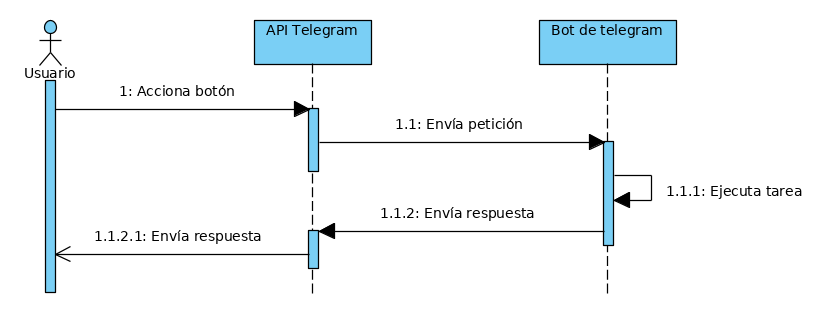
\includegraphics[scale=0.6]{images/84}
	\caption{Interacción usuario con el bot de Telegram}
	\label{f:1}
\end{figure}

Cuando el usuario acciona un botón en la interfaz del bot o envía un comando, dicho mensaje es enviado a la API de Telegram a la cual se conecta el Bot de Telegram gracias al \texttt{API Token}. Dicha solicitud es recibida por el bot desarrollado, que ejecuta la tarea y envía la respuesta a la API de Telegram, y esta a su vez la reenvía a la conversación del bot con el usuario.

\textbf{Proceso de autenticación en el bot de Telegram}

Como se ha podido observar en la figura \ref{f:1}, el usuario ha podido establecer una comunicación con el bot de Telegram, pero para ello es necesario que ese usuario esté registrado como usuario permitido.

En la siguiente figura vamos a observar como se realiza dicho proceso.

\begin{figure}[H]
	\centering
	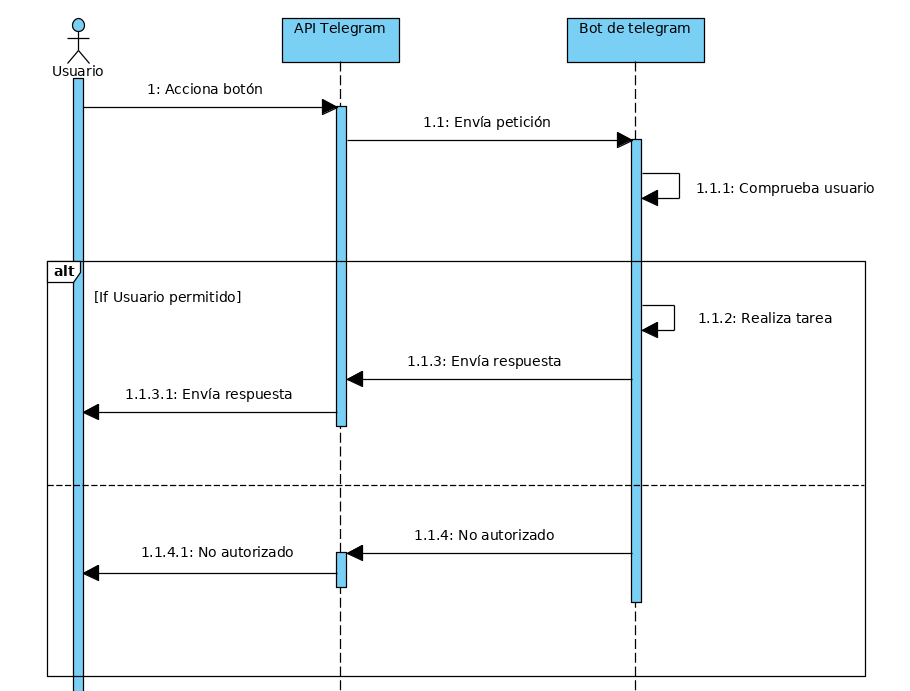
\includegraphics[scale=0.6]{images/85}
	\caption{Interacción usuario autenticado con el bot de Telegram}
	\label{f:2}
\end{figure}

Como se puede observar, cuando el usuario establece una comunicación con el bot, automáticamente se comprueba si dicho usuario está permitido, en cuyo caso se realiza la tarea y se le envía la respuesta. En caso contrario, se le enviará un mensaje diciéndole que no está autorizado.

\textbf{Proceso de autenticación en la API principal}

Una vez el usuario ha establecido comunicación con el bot de Telegram, es necesario que este bot junto con otros servicios se puedan comunicar con la \texttt{API} principal para poder realizar las tareas solicitadas.

Para poder establecer esta comunicación, la \texttt{API} dispone de un sistema de autenticación propio basado en un usuario y contraseña. Dicho usuario y contraseña será necesario adjuntarla junto con la petición a la \texttt{API} para poder establecer dicha comunicación satisfactoriamente.

\begin{figure}[H]
	\centering
	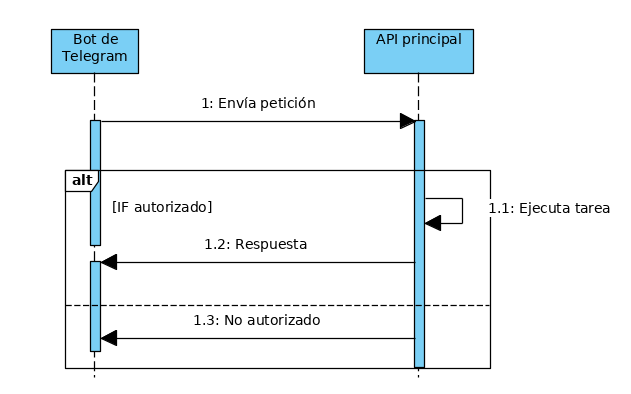
\includegraphics[scale=0.6]{images/86}
	\caption{Interacción entre el bot de Telegram y la API principal}
	\label{f:3}
\end{figure}

Al igual que en el caso anterior, solo se realizará la tarea si el servicio se ha autenticado correctamente, y en caso contrario, se devolverá un mensaje con código de estado 401 (No autorizado).

\textbf{Activación manual de la cámara o vídeo}

Cuando el usuario activa el modo manual para poder realizar una captura de una foto o la grabación de un vídeo, ocurre lo siguiente:

\begin{figure}[H]
	\centering
	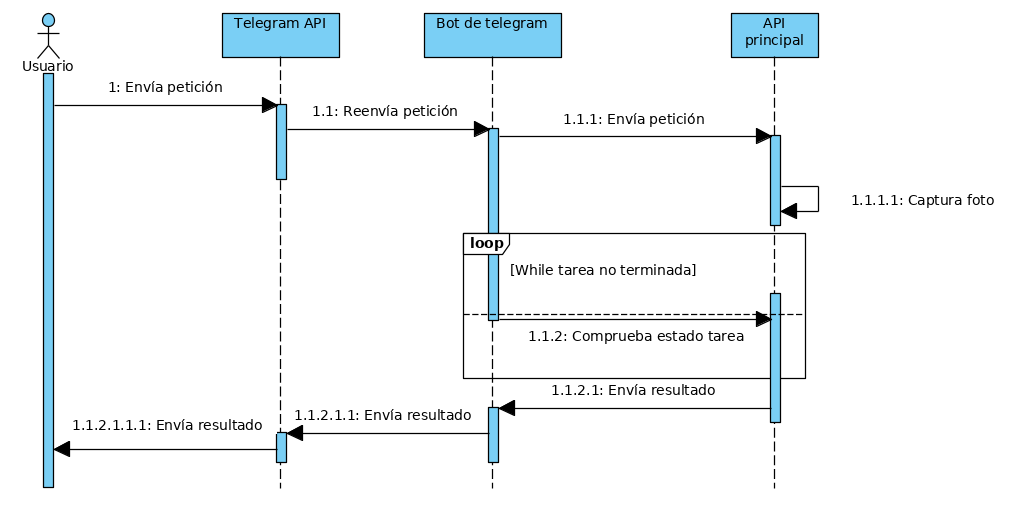
\includegraphics[scale=0.6]{images/87}
	\caption{Interacción entre servicios para realizar una foto}
	\label{f:4}
\end{figure}

Como se puede ver en la figura \ref{f:4}, el bot de Telegram envía la solicitud a la \texttt{API} principal y posteriormente envía periódicamente peticiones a la API para comprobar el estado de la tarea (ya que es asíncrona). Por otra parte, cuando la \texttt{API} recibe la petición para capturar la foto o grabar un vídeo, ésta crea una tarea asíncrona y la pone en cola para poder realizarla. Una vez que ha sido realizada, el bot de Telegram comprobará el estado finalizado y enviará el resultado (que es un mensaje más la imagen capturada) al usuario en la conversación que tiene con el bot.

\textbf{Activación del modo automático}

Cuando el usuario activa el modo automático para poder recibir alertas, ocurre lo siguiente:

\begin{figure}[H]
	\centering
	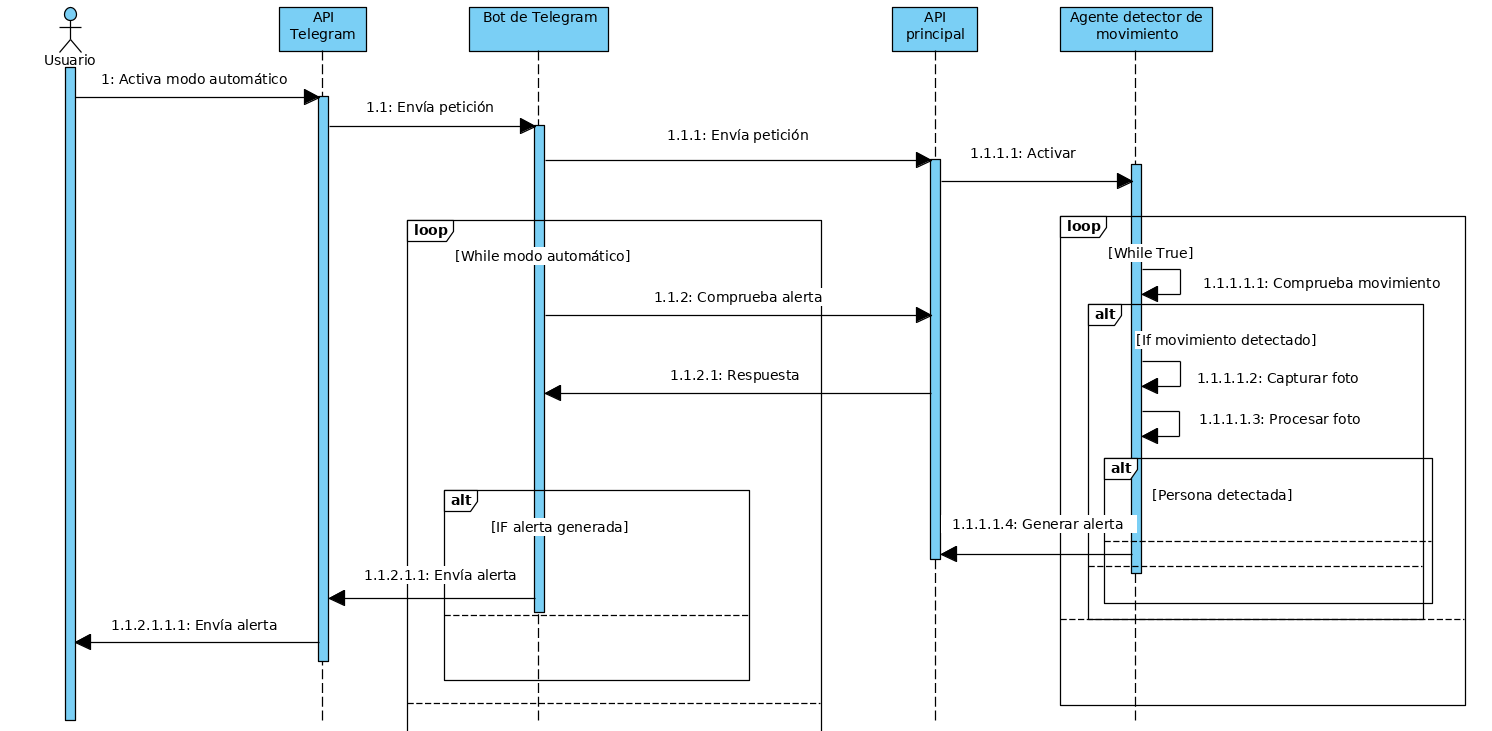
\includegraphics[scale=0.42]{images/88}
	\caption{Interacción entre procesos en el modo automático}
	\label{f:5}
\end{figure}

En primer lugar, la petición llega hasta la \texttt{API} que es la encargada de iniciar el proceso del agente detector de movimiento. A continuación, dicho agente estará en un bucle comprobando el estado del sensor. Cuando se ha detectado algún tipo de movimiento, entonces el agente detector de movimiento realizará una captura de imagen (o vídeo si prefiere) y a continuación pasa a procesar la foto (en el caso de estar habilitada dicha opción). Dicho procesamiento lo realizará el agente detector de objetos (que se detallará en el siguiente apartado) y devolverá la respuesta al agente detector de movimiento. En caso de que se haya detectado una persona, entonces se generará una alerta en la \texttt{API} principal para modificar su estado. Este estado es comprobado periódicamente por el Bot de Telegram, que en cuanto detecte la presencia de una alerta, enviará un mensaje junto con el archivo generado automáticamente (foto o vídeo) al usuario.

También, como observación adicional, se puede comprobar que el bot de Telegram permanece en un bucle realizando peticiones de comprobación a la \texttt{API principal}, pero esto no impide que el bot pueda procesar (en otra hebra) otro tipo de peticiones que se le envíen. De hecho, tiene que atender la petición de cambio de modo para que no se produzca ningún interbloqueo.

\textbf{Interacción entre el agente detector de movimiento y objetos}

Como se ha podido observar en el apartado anterior (ver figura \ref{f:5}), cuando se detecta una alerta de movimiento entonces realiza la captura de una foto y después se pasa a procesarla. El agente detector de objetos es el encargado de realizar este procesamiento. En la siguiente figura se puede observar este proceso.

\begin{figure}[H]
	\centering
	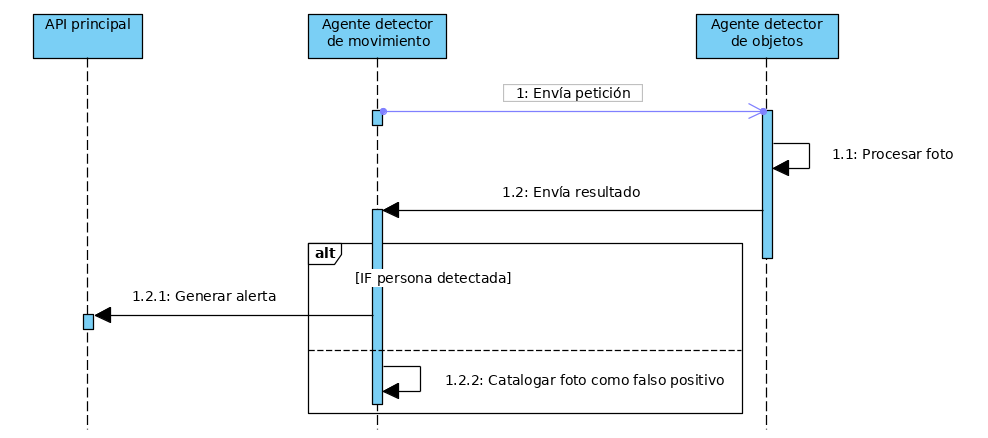
\includegraphics[scale=0.42]{images/90}
	\caption{Interacción entre el agente detector de movimiento y objetos}
	\label{f:6}
\end{figure}

En primer lugar, el agente detector de movimiento envía una petición asíncrona para procesar la foto capturada al agente detector de objetos. Es importante que esta petición sea \textbf{asíncrona}, ya que el procesamiento de la foto puede tardar entre unos 5 y 10 segundos y esto bloquearía al agente detector de objetos para poder seguir capturando posibles alertas.

En cuanto el agente detector de objetos recibe la respuesta, crea pone y en cola dicha tarea para poder ejecutarla. Tras finalizar su ejecución, enviará el resultado al agente detector de movimiento, que comprobará si en ese resultado se ha detectado a una persona. En el caso de detectar una persona, generará una alerta en la \texttt{API} principal, y en caso contrario, catalogará dicha alerta como falsa positiva (o no generará ninguna alerta en la \texttt{API}) y moverá la foto capturada al directorio de archivos falsos positivos.

\textbf{Activación manual del modo streaming}

Cuando el usuario activa el modo streaming para poder visualizar la retransmisión de vídeo en directo, ocurre lo siguiente:

\begin{figure}[H]
	\centering
	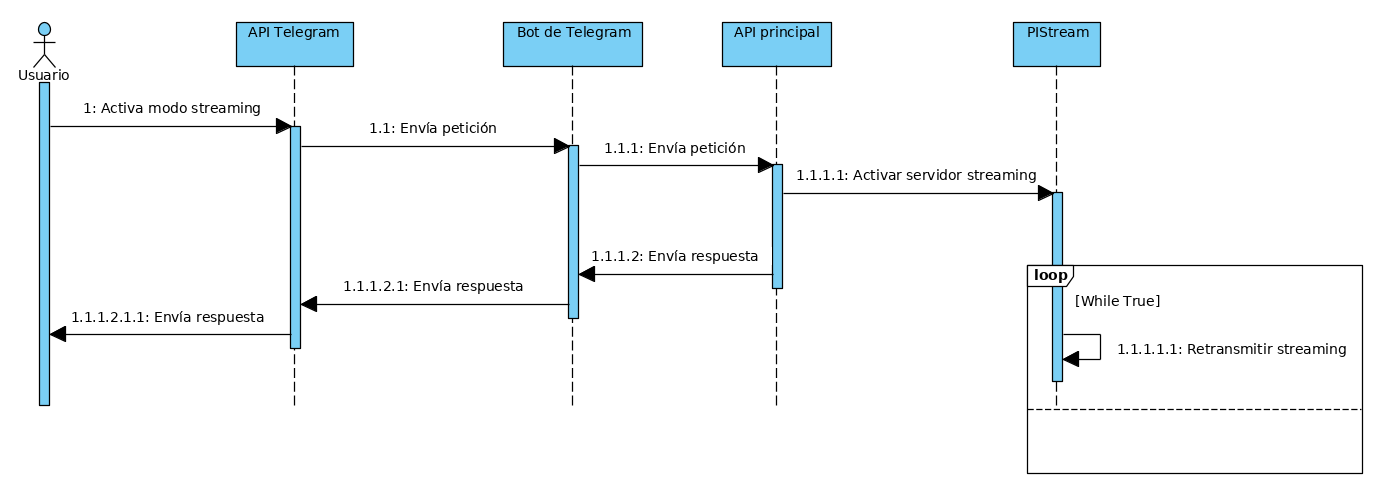
\includegraphics[scale=0.42]{images/89}
	\caption{Interacción entre procesos en el modo streaming}
	\label{f:7}
\end{figure}

En definitiva, el proceso es bastante similar que cuando se activa el modo manual para realizar una captura de una foto o la grabación de un vídeo. En este caso, la \texttt{API} principal se encarga de iniciar el servicio de streaming, que estará continuamente retransmitiendo los datos de vídeo hasta que se vuelva a cambiar de modo. Una vez que este servicio se ha activado, se le envía un mensaje al usuario para notificarle la URL donde podrá visualizar dicho streaming.



\fancypagestyle{miEstilo504}{
   \lhead{5.4 Descripción de la aplicación}
   \rhead{Página \thepage}
   \lfoot{}
   \cfoot{}
   \rfoot{}
}

\pagestyle{miEstilo504}


\subsection{Medidas de seguridad}

Cuando hablamos de un sistema de videovigilancia hay que tener claro que la información grabada por la cámara es de carácter sensible, ya que puede invadir la privacidad de un conjunto de personas, y por lo tanto, hay que controlar quién tiene acceso a dicha información y qué mecanismos se utilizan para que cualquier persona no autorizada no pueda acceder a dicha información.

Además, dado que esta implementación hace uso de un bot de telegram, y dicho bot puede ser de carácter público, hay que tener incluso más cuidado, ya que no se quiere que ningún desconocido pueda tener control sobre nuestro sistema de seguridad que está vigilando nuestro entorno. Por ello, se ha provisto a la aplicación de unos mecanismos de identificación y autenticación simples pero efectivos.

\textbf{Primera medida de seguridad: API token}

En primer lugar, cuando el usuario crea el bot a través del \texttt{BotFather} \cite{ref31}, además de añadir un nombre, descripción \ldots al bot, se le proporciona un \texttt{API token} que consta de una serie de caracteres alfanuméricos, y que debe de ser almacenado como una contraseña. Dicho \texttt{API token} es necesario utilizarlo para configurar el servicio de bot de telegram más adelante. 


\begin{figure}[h]
	\centering
	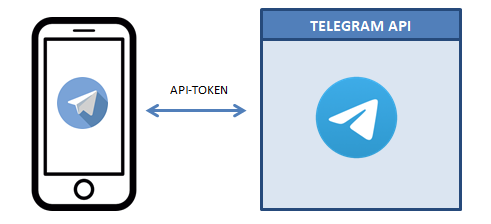
\includegraphics[scale=0.35]{images/36}
	\caption{Primera medida de seguridad}
	\label{img:seg1}
\end{figure}

Esta es la medida que nos aporta la aplicación de telegram para controlar el usuario que pueda administrar dicho bot.

El \texttt{API token} no permite la gestión del bot, pero por ahora si está permitido poder utilizar dicho bot y acceder a su conjunto de funcionalidades, por lo que esto sería un potencial riesgo.

Para prevenir este posible riesgo se ha implementado una segunda medida.

\textbf{Segunda medida: Lista blanca de usuarios}

Esta medida se basa en la implementación de una lista blanca que contiene los identificadores únicos de los usuarios que tienen permiso para utilizar el bot. Esta lista blanca está ubicada en el servicio del bot de telegram, y almacena los identificadores y nombres de usuario permitidos.

\begin{figure}[h]
	\centering
	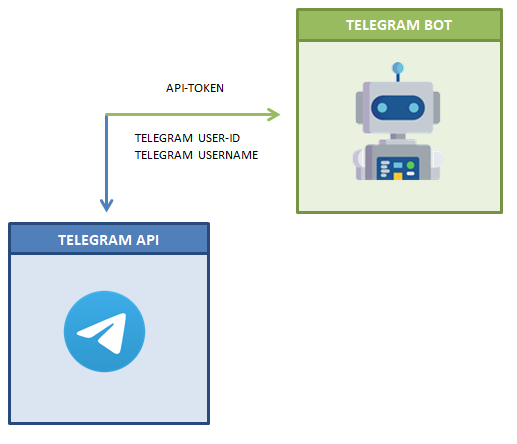
\includegraphics[scale=0.5]{images/37}
	\caption{Segunda medida de seguridad: Lista blanca de usuarios}
	\label{img:seg2}
\end{figure}

Con esta segunda medida, podemos permitir a los usuarios que queramos que tengan acceso a dicha información. Un ejemplo de esta lista blanca es el siguiente:

\vspace{-0.5cm}

\begin{verbatim}
  allowed_users = {
  				    'users':
		                 [
		                   {'id': telegram_user_id, 'username': telegram_username}, 
		                   {'id': bot_user_id, 'username': bot_username}
		                 ]
	              }
\end{verbatim}

\vspace{-0.5cm}


Si un usuario no permitido accede al bot e intenta utilizarlo se le mostrará el siguiente mensaje:

\vspace{-0.5cm}

\begin{verbatim}
You have not permission to access to this content
\end{verbatim}

\vspace{-0.5cm}

También, es importante destacar, que la \textbf{información} que viaja desde que el usuario accede a telegram, hasta que llega al servicio del bot de telegram \textbf{va cifrada}.

Las medidas aplicadas anteriormente sirven para controlar el acceso por parte de la aplicación de telegram, pero ¿y si alguna aplicación externa no autorizada intenta acceder a la \texttt{API} principal?

\texttt{Tercera medida: Autenticación usuario-contraseña}

El tercer mecanismo se basa en restringir el acceso a la \texttt{API} principal de la aplicación a través de una autenticación mediante usuario y contraseña. Esta autenticación la proporciona el módulo \texttt{authentication}, y se basa en comprobar si las credenciales de acceso son correctas,y por lo tanto, la \texttt{API} responderán a las peticiones recibidas.

Estas credenciales de acceso son necesarias para todos los servicios que quieran interactuar con la API, por lo tanto, deben de ser especificadas en el archivo de configuración \texttt{ 	authentication.yml} como se muestra a continuación:

\vspace{-0.5cm}

\begin{verbatim}
---

authentication:
    user: user
    password: sha256$tazHE31s$b4b54292237636e798e407dc935651f9af64a

\end{verbatim}

\vspace{-1cm}

Nótese que la contraseña está cifrada utilizando el algoritmo \texttt{sha256}. Para poder generar este hash, se ha proporcionado un script llamado \texttt{generate\_hash\_password.py} (ubicado en el directorio tools) para poder introducir la contraseña deseada, y se nos devuelve el hash de la contraseña.

En la siguiente figura, podemos observar como todos los servicios interaccionan con la \texttt{API} mediante un usuario y contraseña (menos con los módulos que los importa directamente).

\newpage

\begin{figure}[h]
	\centering
	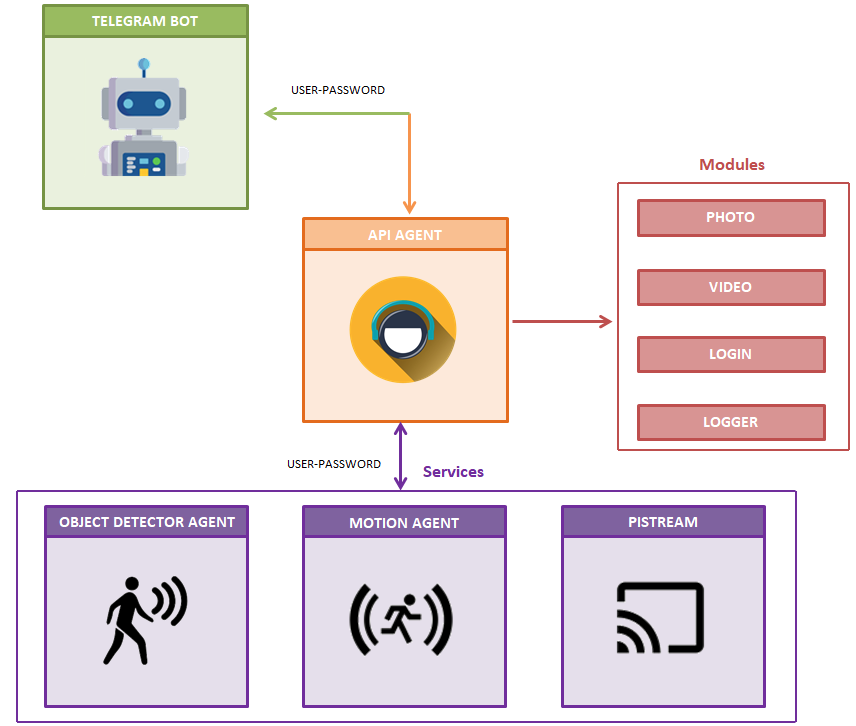
\includegraphics[scale=0.5]{images/38}
	\caption{Tercera medida de seguridad: Usuario y contraseña}
	\label{img:seg3}
\end{figure}




\fancypagestyle{miEstilo505}{
   \lhead{5.5 Interfaz de usuario}
   \rhead{Página \thepage}
   \lfoot{}
   \cfoot{}
   \rfoot{}
}

\pagestyle{miEstilo505}

\subsection{Interfaz de usuario}

Para facilitar la interacción del usuario con la aplicación y mejorar su experiencia de usuario, se ha realizado un diseño de interfaz mediante botones e iconos (interfaz soportada por la API de Telegram) utilizando los llamados 'Callback buttons` \cite{refx1}. Cuando un usuario pulsa estos botones, no se envía ningún mensaje al chat, sino que en su lugar el bot recibe una consulta que es manejada y respondida con una acción.

El diseño propuesto se basa en un modelo jerárquico, donde podremos ir realizando una navegación entre menús partiendo del menú principal.

Este diseño es el siguiente:

\newpage


\begin{figure}[h]
	\centering
	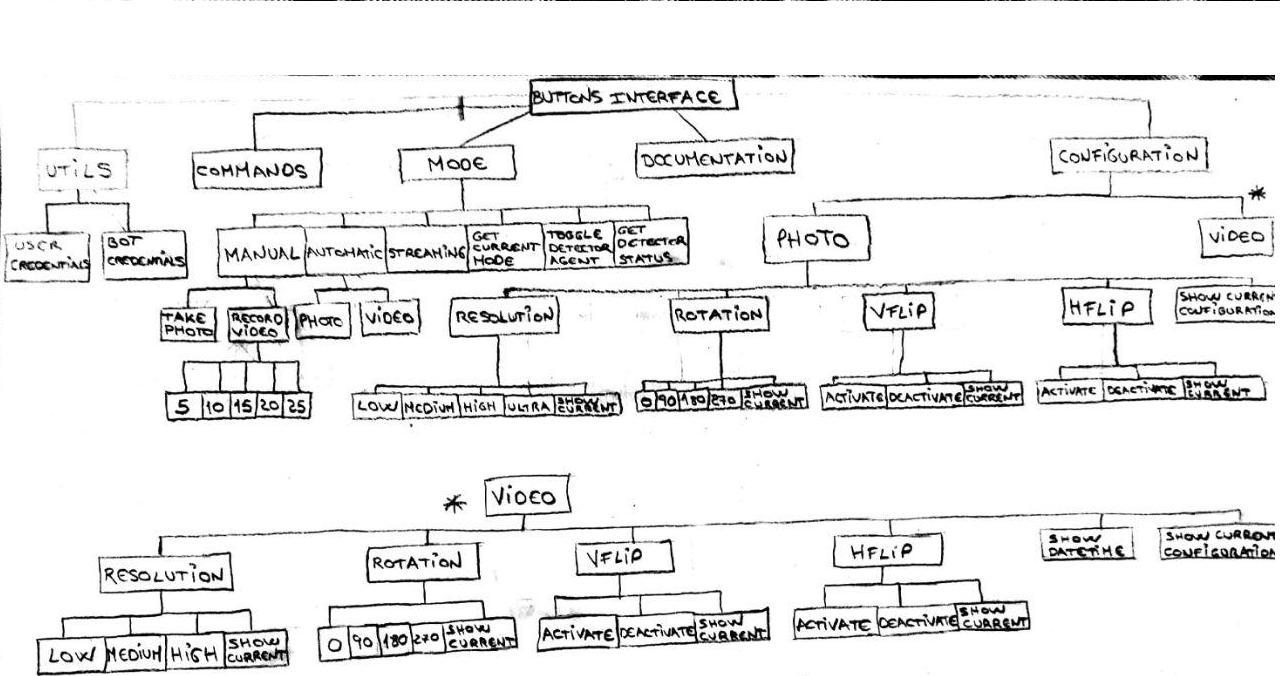
\includegraphics[scale=0.5]{images/55}
	\caption{Diseño de la estructura de la interfaz}
\end{figure}

Su implementación se basa en realizar un menú con un conjunto de botones con los que poder navegar. Por ejemplo, la siguiente figura muestra el menú principal, donde se puede acceder al conjunto de funcionalidades de la aplicación.

\begin{figure}[h]
	\centering
	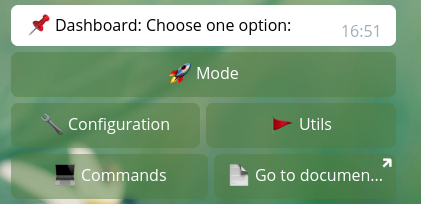
\includegraphics[scale=0.8]{images/42}
	\caption{Menú principal de la aplicación}
\end{figure}

En la sección de \textit{Mode} se podrá acceder al conjunto de acciones relacionadas con los modos de uso de la aplicación, en \textit{Configuration} se podrá acceder al conjunto de opciones para configurar la cámara \ldots
Por ejemplo, si pulsamos el botón de \textit{Mode} se podrá acceder al conjunto de funcionalidades relacionadas.

\begin{figure}[h]
	\centering
	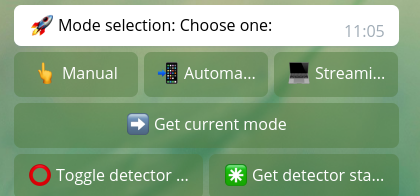
\includegraphics[scale=0.8]{images/39}
	\caption{Menú Mode}
\end{figure}

La implementación de esta interfaz se puede comprobar en este \href{https://github.com/jmv74211/TFM_security_system_PI/blob/master/src/agents/telegram_bot.py#L972}{enlace}.

\begin{tabular}{|p{15.5cm}|}
	
	\hline
	
	\textit{ \textbf{*Nota:} Para más información, todo este conjunto de botones y funcionalidades serán explicados en la guía de usuario de la sección \ref{anex:guia}. }
	\\
	\hline
	
\end{tabular}





\fancypagestyle{miEstilo506}{
   \lhead{5.6 Descripción de archivos y directorios}
   \rhead{Página \thepage}
   \lfoot{}
   \cfoot{}
   \rfoot{}
}

\pagestyle{miEstilo506}


\subsection{Descripción de archivos y directorios}

La aplicación \texttt{SIVIRA} está compuesta por una serie de archivos y directorios que implementan y ejecutan el conjunto de servicios del sistema de videovigilancia.

Todos estos archivos y directorios están disponibles en el repositorio oficial del proyecto en Github \cite{ref1}.

\begin{figure}[h]
	\centering
	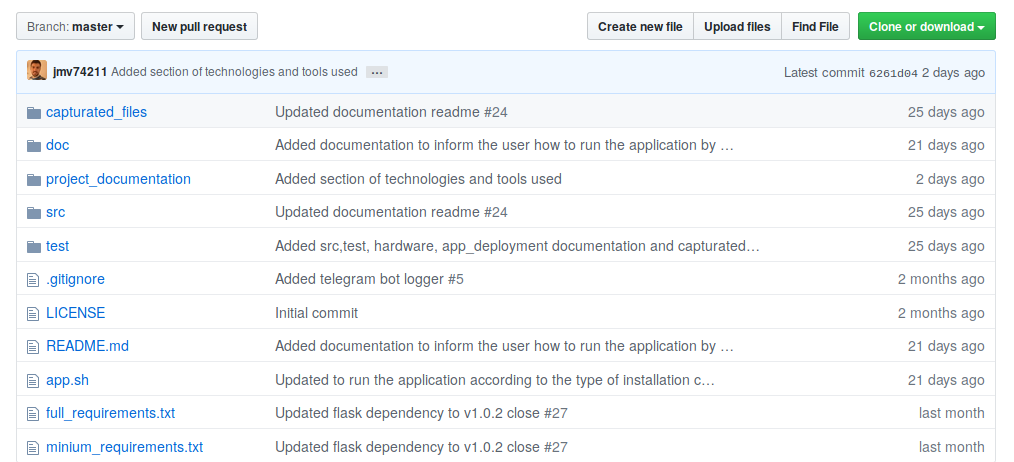
\includegraphics[scale=0.5]{images/43}
	\caption{Repositorio de Github del proyecto SIVIRA}
\end{figure}

A continuación, se explicará cómo se ha organizado todos estos archivos y directorios, junto con una breve descripción sobre el objetivo de cada uno.

\textbf{Capturated\_files}

Este directorio está destinado a almacenar el conjunto de archivos de imágenes y vídeo generados por el sistema de videovigilancia. Su estructura es la siguiente puede verse en la figura \ref{fig:tik1}.

Se compone de los siguientes elementos:

\vspace{-0.5cm}

\begin{itemize}
\item \textbf{alerts}: Directorio donde se almacenan todos los archivos generados mediante alertas (capturas o grabaciones automáticos tras ser activado el sensor de movimiento).

	\begin{itemize}
	\item \textbf{false\_positive}: Directorio donde serán almacenados todos los archivos generados tras ser activado el sensor de movimiento y que el agente detector de objetos ha filtrado tras comprobar que no hay ninguna persona en dichas fotos.
	\end{itemize}

\item \textbf{photos}: Directorio donde se almacenan todas las fotos capturadas de forma manual.

\item \textbf{videos}: Directorio donde se almacenan todas los vídeos capturados de forma manual.

\item \textbf{Readme.md}: Archivo de documentación para el repositorio.

\end{itemize}



\tikzstyle{every node}=[draw=black,thick,anchor=west]
\tikzstyle{selected}=[draw=red,fill=red!30]
\tikzstyle{optional}=[dashed,fill=gray!50]

\begin{figure}[H]
\centering

\begin{tikzpicture}[%
  grow via three points={one child at (0.5,-0.7) and
  two children at (0.5,-0.7) and (0.5,-1.4)},
  edge from parent path={(\tikzparentnode.south) |- (\tikzchildnode.west)}]
  \node {SIVIRA\_APP}
    child { node {capturated\_files}
		  child { node {alerts}
		  		child { node {false\_positive}}
		  }
		  child [missing] {}	
          child { node {photos}}
          child { node {videos}}
          child { node {README.md}}     
    }
    child [missing] {}	
    child [missing] {}	
    child [missing] {}	
    child [missing] {}	
    child [missing] {}	
    child { node {\ldots}};
   
\end{tikzpicture}
\caption{Estructura de directorios de capturated\_files} \label{fig:tik1}
\end{figure}

\textbf{Doc}

Este directorio contiene una estructura de archivos de documentación en formato \texttt{.md} para que puedan ser consultados desde el repositorio de Github. Su estructura es la siguiente puede verse en la figura \ref{fig:tik2}.

\begin{figure}
\centering
\begin{tikzpicture}[%
  grow via three points={one child at (0.5,-0.7) and
  two children at (0.5,-0.7) and (0.5,-1.4)},
  edge from parent path={(\tikzparentnode.south) |- (\tikzchildnode.west)}]
  \node {SIVIRA\_APP}
  	child { node {\ldots}}
    child { node {doc}
		  child { node {api}
		  		child { node {README.md}}
		  		child { node {api\_agent\_doc.md}}
		  		child { node {object\_detector\_agent\_doc.md}}
		  }
		  child [missing] {}
		  child [missing] {}
		  child [missing] {}
		  child [missing] {}	
          child { node {app\_deployment}
          		child { node {README.md}}
          }
          child [missing] {}
          child { node {backend\_app}
                child { node {README.md}}
          }
          child [missing] {}
          child { node {hardware}
                child { node {README.md}}
          }
          child [missing] {}
          child { node {images}
                child { node {\ldots}}
          }
		  child [missing] {}
          child { node {installation}
                child { node {README.md}}
          }  
		  child [missing] {}
          child { node {test}
                child { node {README.md}}
          }
          child [missing] {} 
		  child [missing] {}
          child { node {user\_guide}
                child { node {README.md}}
          }         
          child [missing] {}           
          child [missing] {}      
          child { node {README.md}}     
    }
    child [missing] {}	
    child [missing] {}	
    child [missing] {}	
    child [missing] {}	
    child [missing] {}
    child [missing] {}
    child [missing] {}
    child [missing] {}
    child [missing] {}
    child [missing] {}
    child [missing] {}
    child [missing] {}
    child [missing] {}
    child [missing] {}
    child [missing] {}
    child [missing] {}
    child [missing] {}
    child [missing] {}
    child [missing] {}
    child [missing] {}
    child [missing] {}
    child [missing] {} 
    child { node {\ldots}};

\end{tikzpicture}
\caption{Estructura de directorios de doc} \label{fig:tik2}
\end{figure}


Se compone de los siguientes elementos:

\vspace{-0.5cm}

\begin{itemize}
\item \textbf{api}: Directorio donde se almacena la documentación de la \texttt{API}.

	\begin{itemize}
	\item \textbf{README.md}: Documentación sobre aplicación y uso de la \texttt{API} y la api del agente detector de objetos.
	\item \textbf{api\_agent\_doc.md}: Documentación sobre aplicación y uso de la \texttt{API} principal.
	\item \textbf{object\_detector\_agent.md}: Documentación sobre aplicación y uso del agente detector de objetos.
	\end{itemize}

\item \textbf{app\_deployment}: Directorio que contiene documentación sobre cómo desplegar y ejecutar la aplicación.

\item \textbf{backend\_app}: Directorio que contiene documentación el contenido del directorio \textit{src}.

\item \textbf{hardware}: Directorio que contiene documentación sobre el hardware necesario, cómo instalarlo y su presupuesto.

\item \textbf{images}: Directorio que contiene las imágenes que se han utilizado en la documentación del repositorio.

\item \textbf{installation}: Directorio que contiene documentación sobre cómo instalar los componentes necesarios para ejecutar la aplicación.

\item \textbf{test}: Directorio que contiene documentación sobre cómo ejecutar los tests de la aplicación.

\item \textbf{user\_guide}: Directorio que contiene documentación sobre cómo utilizar las distintas funcionalidades de la aplicación a través de la interfaz del bot de telegram.

\item \textbf{Readme.md}: Archivo que contiene el índice general sobre la distinta documentación disponible.

\end{itemize}

\textbf{Project documentation}

Este directorio contiene el conjunto de archivos necesarios para generar la documentación del proyecto (este fichero pdf). Su estructura es la siguiente puede verse en la figura \ref{fig:tik3}.

\begin{figure}
\centering
\begin{tikzpicture}[%
  grow via three points={one child at (0.5,-0.7) and
  two children at (0.5,-0.7) and (0.5,-1.4)},
  edge from parent path={(\tikzparentnode.south) |- (\tikzchildnode.west)}]
  \node {SIVIRA\_APP}
  	child { node {\ldots}}
    child { node {project\_documentation}
    	  child [missing] {}
		  child { node {images}
		  		child { node {\ldots}}
		  }
		  child [missing] {}
		  child { node {src}
		  		child { node {\ldots}}
		  }
		  child [missing] {}
          child { node {documentation.text}}        
    }
    child [missing] {}	
    child [missing] {}
    child [missing] {}
    child [missing] {}	
    child [missing] {}	
    child [missing] {}
    child { node {\ldots}};

\end{tikzpicture}
\caption{Estructura de directorios de project\_documentation} \label{fig:tik3}
\end{figure}

Se compone de los siguientes elementos:

\vspace{-0.5cm}

\begin{itemize}
\item \textbf{images}: Directorio donde se almacenan las imágenes utilizadas para realizar esta documentación del proyecto.
\item \textbf{src}: Directorio donde se almacenan los archivos fuentes \texttt{.text} que se necesitan para compilar y generar la documentación del proyecto.
\item \textbf{documentation.text}: Archivo Látex que contiene toda la documentación del proyecto a partir del resto de archivos fuentes.
\end{itemize}

\textbf{SRC: Directorio de archivos fuentes}

Este directorio contiene el conjunto de archivos fuentes necesarios para construir la aplicación \texttt{SIVIRA}. Su estructura es la siguiente puede verse en la figura \ref{fig:tik4}.

Se compone de los siguientes elementos:

\vspace{-0.5cm}

\begin{itemize}
\item \textbf{agents}: Directorio donde se almacenan todos los archivos fuentes de los procesos y servicios de la aplicación. Estos son:

	\begin{itemize}
	\item \textbf{API\_agent.py}: Servicio que inicia la \texttt{API} principal de la aplicación.
	\item \textbf{motion\_agent.py}: Servicio que inicia el reconocimiento de movimiento a través del sensor y genera alertas en la \texttt{API} principal.
	\item \textbf{object\_detector\_agent.py}: Servicio que inicia una api secundaria para poder realizar el reconocimiento de objetos en una foto con el objetivo de poder filtrar las alertas generadas por el \texttt{motion\_agent}.
	\item \textbf{telegram\_bot.py}: Servicio que inicia el bot de telegram que hace de intermediario entre la aplicación de telegram usada por el usuario y la \texttt{API} principal.
	\end{itemize}

\item \textbf{config}: Directorio donde se almacenan archivos de configuración modificados por el usuario y necesarios para configurar correctamente la aplicación. Estos son:

	\begin{itemize}
	\item \textbf{authentication.yml}: Archivo de configuración donde se introducen las credenciales utilizadas para poder comunicarse y enviar peticiones a la \texttt{API}.
	\item \textbf{modules\_config.yml}: Archivo de configuración que contiene los parámetros por defecto para la cámara y grabación de vídeo (resolución, rotación \ldots) y que el usuario puede modificar a través del bot de telegram.
	\item \textbf{telegram\_config.yml}: Archivo de configuración que contiene las credenciales de acceso necesarias para comunicarse con el bot de telegram y la \texttt{API} de la aplicación.
	\end{itemize}

\item \textbf{lib}: Directorio donde se almacenan archivos que contienen funciones auxiliares a utilizar por los componentes de la aplicación. En este caso solo contiene un archivo, pero en versiones posteriores podrá contener más archivos.

	\begin{itemize}
	\item \textbf{flask\_celery.py}: Contiene funciones auxiliares para la configuración de la gestor de tareas \texttt{celery} \cite{ref15} en \texttt{Flask} \cite{ref14}.
	\end{itemize}

\item \textbf{modules}: Directorio donde se almacenan todos los archivos correspondientes a las implementaciones de los módulos que utilizarán el resto de servicios y \texttt{API} para conectarse con el recurso de la cámara, generar logs \ldots Estos módulos son:

	\begin{itemize}
	\item \textbf{object\_detector}: Contiene el conjunto de directorios y dependencias necesarias que importa el servicio detector de objetos.
	\item \textbf{pistream}: Contiene el conjunto de ficheros necesarios para ejecutar el servicio de streaming. Está compuesto por los siguientes elementos:
		\begin{itemize}
		\item \textbf{README.md}: Documentación del repositorio original que se ha usado y modificado para implementar este servicio.
		\item \textbf{index.html}: Contiene la página web responsive donde se reproducirá la imagen de streaming.
		\item \textbf{jsmpg.js}: Contiene el conjunto de funciona de Javascript que importa el servidor web de streaming.
		\item \textbf{streaming\_server.py}: Contiene la implementación del servidor de streaming.
		\end{itemize}
		
		\item \textbf{authentication.py}: Archivo que implementa el módulo de autenticación usado por la \texttt{API}.
		\item \textbf{logger.py}: Archivo que implementa el módulo de logs que es usado por el resto de servicios de la aplicación.
		\item \textbf{photo.py}: Fichero que implementa las funcionalidades necesarias para comunicarse el recurso hardware de la cámara para realizar fotos.
		\item \textbf{video.py}: Fichero que implementa las funcionalidades necesarias para comunicarse el recurso hardware de la cámara para grabar vídeos.
				
	\end{itemize}

\item \textbf{tools}: Directorio cuyo objetivo es almacenar pequeñas aplicaciones o herramientas que realicen alguna tarea útil en concreto. En este caso, solo existe el siguiente fichero:
	\begin{itemize}
	\item \textbf{generate\_hash\_password.py}: Pequeño script para generar el hash de una contraseña. El usuario introduce por consola su contraseña en texto plano y se le devuelve el hash cifrado con sha512.
	\end{itemize}

\item \textbf{README.md}: Archivo de documentación del repositorio de Github que describe brevemente el contenido de la carpeta de \textit{src}.

\item \textbf{settings.py}: Archivo de configuración genérico de la aplicación. En este archivo se configuran los parámetros globales que utilizará la aplicación (direcciones IP, puertos \ldots).

\end{itemize}

\begin{figure}[H]
\centering
\begin{tikzpicture}[%
  grow via three points={one child at (0.5,-0.7) and
  two children at (0.5,-0.7) and (0.5,-1.4)},
  edge from parent path={(\tikzparentnode.south) |- (\tikzchildnode.west)}]
  \node {SIVIRA\_APP}
  	child { node {\ldots}}
    child { node {src}
    	  child [missing] {}
		  child { node {agents}
		  		child { node {api\_agent.py}}
	  			child { node {motion\_agent.py}}
  				child { node {object\_detector\_agent.py}}
  				child { node {telegram\_bot.py}}
		  }
		  child [missing] {}
		  child [missing] {}
		  child [missing] {}
		  child [missing] {}
		  child [missing] {}
		  child { node {config}
		  		child { node {authentication.yml}}
		  		child { node {modules\_config.yml}}
		  		child { node {telegram\_config.yml}}
		  }
		  child [missing] {}
		  child [missing] {}
		  child [missing] {}
          child { node {lib}
          		child { node {flask\_celery.py}}
          } 
          child [missing] {}
          child [missing] {}
          child { node {modules}
   		  		child { node {object\_detector}
   		  				child { node {\ldots}}
   		  		}
   		  		child [missing] {}
   		  		child { node {pistream}
		  			child { node {README.md}}
   		  			child { node {index.html}}
					child { node {jsmpg.js}}
		   			child { node {streaming\_server.py}}
   		  		}
   		  		child [missing] {}	
   		  		child [missing] {}	
   		  		child [missing] {}	
   		  		child [missing] {}	
   		  		child [missing] {}	
   		  		child { node {authentication.py}}
   		  		child { node {logger.py}}
   		  		child { node {photo.py}}
   		  		child { node {video.py}}
		  }
		  child [missing] {}
		  child [missing] {}
		  child [missing] {}
		  child [missing] {}
		  child [missing] {}
		  child [missing] {}
		  child [missing] {}
		  child [missing] {}
		  child [missing] {}
		  child [missing] {}
		  child [missing] {}
		  child [missing] {}
		  child { node {tools}
	  		child { node {generate\_hash\_password.py}}
	  	  }
	  	  child [missing] {}
	  	  child [missing] {}
	  	  child { node {settings.py}}
	  	  child { node {README.md}}  
    }
    child [missing] {}	
    child [missing] {}
    child [missing] {}
    child [missing] {}	
    child [missing] {}	
    child [missing] {}
    child [missing] {}
    child [missing] {}
    child [missing] {}
    child [missing] {}
    child [missing] {}
    child [missing] {}
    child [missing] {}
    child [missing] {}
    child [missing] {}
    child [missing] {}
    child [missing] {}
    child [missing] {}
    child [missing] {}
    child [missing] {}
    child [missing] {}
    child [missing] {}
    child [missing] {}
    child [missing] {}
    child [missing] {}
    child [missing] {}
    child [missing] {}
    child [missing] {}
    child [missing] {}
    child [missing] {}
    child [missing] {}
    child [missing] {}
    child { node {\ldots}};

\end{tikzpicture}
\caption{Estructura de directorios de src} \label{fig:tik4}
\end{figure}

\textbf{Test}

Este directorio contiene el conjunto de archivos necesarios para ejecutar los test unitarios e integración para probar el correcto funcionamiento de los módulos de la aplicación. Su estructura es la siguiente puede verse en la figura \ref{fig:tik5}.

Se compone de los siguientes elementos:

\vspace{-0.5cm}

\begin{itemize}
\item \textbf{integration}: Directorio donde se almacenan los test de integración. Estos son:

	\begin{itemize}
	\item \textbf{test\_api\_agent.py}: Contiene el conjunto de tests que hacen uso de peticiones HTTP para poder probar el conjunto de funcionalidades de la \texttt{API}.
	\item \textbf{test\_object\_detector\_agent.py}: Contiene el conjunto de tests que hacen uso de peticiones HTTP para poder probar el conjunto de funcionalidades del agente detector de objetos.
	\end{itemize}

\item \textbf{unit}: Directorio donde se almacenan los test unitarios. Estos son:

	\begin{itemize}
	\item \textbf{test\_api\_agent.py}: Contiene el conjunto de tests que prueban las funciones implementadas por la \texttt{API}.
	\item \textbf{test\_authentication.py}: Contiene el conjunto de tests para probar la funcionalidades del módulo de autenticación.
	\item \textbf{test\_logger.py}: Contiene el conjunto de tests para probar la funcionalidades del módulo de logs.
	\item \textbf{test\_motion\_agent.py}: Contiene el conjunto de tests para probar la funcionalidades del agente detector de movimiento.
	\item \textbf{test\_object\_detector.py}: Contiene el conjunto de tests para probar la funcionalidades del agente detector de objetos.
	\item \textbf{test\_photo.py}: Contiene el conjunto de tests para probar las funcionalidades del módulo Photo.
	\item \textbf{test\_photo.py}: Contiene el conjunto de tests para probar las funcionalidades del módulo Camera.
	\end{itemize}

\item \textbf{README.md}: Archivo que contiene documentación con ejemplos para poder ejecutar los test.

\begin{figure}[H]
\centering

\begin{tikzpicture}[%
  grow via three points={one child at (0.5,-0.7) and
  two children at (0.5,-0.7) and (0.5,-1.4)},
  edge from parent path={(\tikzparentnode.south) |- (\tikzchildnode.west)}]
  \node {SIVIRA\_APP}
  	child { node {\ldots}}
    child { node {test} 	
    	  child [missing] {}
		  child { node {integration}
		  		child { node {test\_api\_agent.py}}
		  		child { node {test\_object\_detector\_agent.py}}
		  }
		  child [missing] {}
		  child [missing] {}
		  child { node {unit}
		  		child { node {test\_api\_agent.py}}
		  		child { node {test\_authentication.py}}
		  		child { node {test\_logger.py}}
		  		child { node {test\_motion\_agent.py}}
		  		child { node {test\_object\_detector.py}}
		  		child { node {test\_photo.py}}
		  		child { node {test\_video.py}}
		  }
		  child [missing] {}
		  child [missing] {}
		  child [missing] {}
		  child [missing] {}
		  child [missing] {}
		  child [missing] {}
		  child [missing] {}
		  child [missing] {}
          child { node {README.md}}        
    }
    child [missing] {}	
    child [missing] {}
    child [missing] {}
    child [missing] {}	
    child [missing] {}	
    child [missing] {}
    child [missing] {}
    child [missing] {}
    child [missing] {}
    child [missing] {}
    child [missing] {}
    child [missing] {}
    child [missing] {}
    child [missing] {}
    child { node {\ldots}};

\end{tikzpicture}
\caption{Estructura de directorios de test} \label{fig:tik5}
\end{figure}

\end{itemize}

\textbf{LICENSE}

Archivo que contiene la descripción de la licencia \textbf{GNU General Public License v3.0} que es bajo la que está respaldada este proyecto.

\textbf{README.md}

Archivo que contiene la página principal de la documentación de la aplicación para el repositorio de Github \cite{ref1}. Contiene una descripción y enlaza con el resto de documentación del directorio \textit{doc}.

\newpage

\textbf{app.sh}

Este archivo contiene un script \texttt{bash} que es el utilizado para iniciar y parar los procesos que ejecutan la aplicación. En la sección X se detalla más sobre cómo utilizar este script.

\textbf{full\_requirements.txt}

Archivo que contiene las dependencias de Python necesarias para instalar todos los componentes y servicios necesarios por la aplicación.

\textbf{minimum\_requirements.txt}

Archivo que contiene las dependencias básicas de Python para realizar una instalación mínima de los componentes y servicios necesarios por la aplicación.



\newpage



\fancypagestyle{miEstilo6}{
   \lhead{6. Presupuesto}
   \rhead{Página \thepage}
   \lfoot{}
   \cfoot{}
   \rfoot{}
}

\pagestyle{miEstilo6}

\section{Presupuesto}

En esta sección se va a realizar un presupuesto estimado y justificado acerca del coste del proyecto. Adicionalmente, se realizará también una estimación de costes y beneficios que conllevaría la puesta en marcha de este proyecto al mercado laboral.

\subsection{Presupuesto desglosado por conceptos}

\begin{table}[H]
\centering
\begin{tabular}{|l|l|}
\hline
\rowcolor[HTML]{4F81BD} 
{\color[HTML]{FFFFFF} \textbf{Gastos elegibles}} & {\color[HTML]{FFFFFF} \textbf{Importe solicitado}} \\ \hline
\rowcolor[HTML]{EFEFEF} 
{\color[HTML]{FE0000} Gasto de personal} & {\color[HTML]{FE0000} 9202\euro} \\ \hline
\hspace{1cm}Total gastos de contratación & {\color[HTML]{F56B00} 9202\euro} \\ \hline
\rowcolor[HTML]{EFEFEF} 
{\color[HTML]{FE0000} Gastos de ejecución} & {\color[HTML]{FE0000} 733.5\euro} \\ \hline
Costes de adquisición de material inventariable & {\color[HTML]{F56B00} 298.5\euro} \\ \hline
\hspace{1cm}1 portátil durante 3 meses & 145\euro \\ \hline
\hspace{1cm}1 Kit Raspberry PI & 55\euro \\ \hline
\hspace{1cm}1 Cámara & 6\euro \\ \hline
\hspace{1cm}1 Sensor de movimiento & 1\euro \\ \hline
\hspace{1cm}1 Caja para la Raspberry PI & 11\euro \\ \hline
\hspace{1cm}1 Cableado & 2.5\euro \\ \hline
\hspace{1cm}1 Licencia 3 meses Visual Paradigm & 18\euro \\ \hline
\hspace{1cm}1 Licencia 3 meses Pycham & 60\euro \\ \hline
Costes de suministros... & {\color[HTML]{F56B00} 435\euro} \\ \hline
\hspace{1cm}Alquiler estancia & 150\euro \\ \hline
\hspace{1cm}Gasto de luz & 90\euro \\ \hline
\hspace{1cm}Gasto de agua & 80\euro \\ \hline
\hspace{1cm}Gasto de internet & 95\euro \\ \hline
\hspace{1cm}Gastos de consumibles varios: Café... & 20\euro \\ \hline
\rowcolor[HTML]{EFEFEF} 
{\color[HTML]{FE0000} Gastos complementarios} & {\color[HTML]{FE0000} 30\euro} \\ \hline
\hspace{1cm}Transporte para reuniones de revisión & 30\euro \\ \hline
\rowcolor[HTML]{EFEFEF} 
\multicolumn{1}{|r|}{\cellcolor[HTML]{EFEFEF}\textbf{Coste total}} & {\color[HTML]{FE0000} 9965.5\euro} \\ \hline
\end{tabular}
\end{table}

\newpage

\subsection{Justificación del presupuesto}

\textbf{Gastos de personal}

El precio hora bruto que se paga a un ingeniero informático se ha establecido en 17\euro

Dado que este proyecto se ha realizado de forma individual, los gastos de contratación se corresponderían solo con la suma del salario bruto más las deducciones a pagar. Dicho salario bruto vendría dado por la siguiente fórmula:

\vspace{-0.7cm}

\[
NºHorasTotales * PrecioHora + SueldoProporcionalVacaciones
\]

El sueldo proporcional a las vacaciones se correspondería con dos días y medio de vacaciones por cada mes trabajado, por lo tanto se calcularía de la siguiente forma:

\vspace{-1cm}

\[
SueldoProporcionalVacaciones =  (3 meses * (2.5 \text{días/mes} *  \text{8h/día})) *17 \text{\euro}/hora = 1020 \text{\euro}
\]

\vspace{-0.3cm}

Si sustituimos los valores dados en la tabla obtenemos lo siguiente:

\vspace{-0.7cm}

\[
\text{\textit{Salario bruto =} }341h*17\text{\euro/h}+1020\text{\euro} = 6817\text{\euro}
\]

Finalmente, el gasto por personal total del proyecto sería:

\vspace{-0.7cm}

\[
\text{\textit{Gasto de personal}} = \text{\textit{salario bruto}} + 35\text{\%} \text{\textit{deducción}} = 6817\text{\euro} + 35\text{\%} = 9202\text{\euro}
\]

\textbf{Gastos de ejecución}

Los costes de ejecución vienen dados por la siguiente fórmula:

$\text{\textit{Coste}} = \text{\textit{cantidad}} * \text{\textit{precio}} * \dfrac{\text{\textit{Tiempo uso}}}{\text{\textit{Periodo amortización}}}$

A continuación se desglosan el conjunto de gastos

\begin{itemize}
\item Portátil = $ 1u* 1750\text{\euro} * (3 meses/36 meses) = 145\text{\euro} $
\item Kit Raspberry PI = $ 1u*55\text{\euro} * 1 = 55\text{\euro} $
\item Cámara = $ 1u* 6\text{\euro} * 1 = 6\text{\euro} $
\item Sensor de movimiento = $ 1u* 1\text{\euro} * 1 = 1\text{\euro} $
\item Caja para la Raspberry PI = $ 1u* 11\text{\euro} * 1 = 11\text{\euro} $
\item Cableado = $ 1u* 2.5\text{\euro} * 1 = 2.5\text{\euro} $
\item Licencia 3 meses Visual Paradigm = $ 1u* 18\text{\euro} = 18\text{\euro} $
\item Licencia 3 meses Pycharm. = $ 1u* 20\text{\euro} = 20\text{\euro} $
\end{itemize}

\begin{tabular}{|p{15.5cm}|}
	
	\hline
	
	\textit{ \textbf{*Nota:} Cuando el resultado del tiempo de uso entre el periodo de amortización vale 1, significa que el uso de dicho componente es únicamente dedicado para este proyecto.}
	\\
	\hline
	
\end{tabular}

\vspace{0.3cm}

Respecto a los gastos de suministros, los precios se han estimado en función de la media total que se pagan por dichos suministros fuera del periodo de desarrollo.

\textbf{Gastos Complementarios}

Durante el desarrollo de este proyecto, se han previsto un total de 3 visitas al cliente (en este caso el tutor del TFM). Se estima alrededor de 1 hora por visita más el gasto de transporte que hacen una estimación total de 30\euro.

\subsection{Estimación de costes y beneficios en el mercado laboral}

En la sección anterior, se ha podido comprobar el coste que ha supuesto el desarrollo de este proyecto, pero ¿qué pasaría si este proyecto se lanzara al mercado laboral?. A continuación se va a realizar una estimación de los costes y beneficios que esto supondría.

Antes de empezar a estimar posibles costes, se ha realizado un estudio acerca de las cuotas mensuales que suelen cobrar las principales compañías de alarmas y videovigilancia, y se ha podido ver que la cuota mensual suele rondar alrededor de los 30-40\euro (Por ejemplo aquí puede verse los \href{https://www.comparaiso.es/alarmas/empresas-seguridad/securitas-direct/precio}{precios de securitas-direct}).

También, mencionar que en un principio, la puesta en marcha y mantenimiento del servicio no supondría ningún coste externo de contratación de servicios (como cloud, licencias \ldots), sino que solo bastaría realizar una inversión inicial en el hardware (Raspberry PI y sus componentes). En base a este dato, se han realizado las siguientes estimaciones.

\textbf{Instalación del servicio}

El coste que supondría realizar la instalación del servicio sería el siguiente:

\begin{itemize}
\item \textbf{Coste real de los componentes}: 71\euro

\item \textbf{Gastos de instalación y desplazamiento}: 15\euro

\end{itemize}

\vspace{-0.4cm}

El presupuesto que se pediría al cliente para realizar la instalación sería de unos 100\euro. En este precio va incluido todo el hardware necesario, que pasaría a ser propiedad del cliente desde el primer momento.

El beneficio en esta etapa sería de \textbf{16\euro} (100 de presupuesto - 86 de coste). Esta cantidad es casi insignificante, y no aporta casi ninguna ganancia, pero el objetivo no es ganar una gran cantidad al realizar la instalación, sino por el mantenimiento del servicio. Por ello se ha intentado reducir el coste inicial con motivo de poder atraer el máximo número de clientes.

\textbf{Mantenimiento del servicio}

El mantenimiento del servicio se basaría en un soporte técnico y de ayuda a los clientes. Los clientes pagarían una cuota mensual a cambio de poder reportar incidencias para que puedan ser ayudados.

Este servicio no supondrá ningún coste externo más allá de la mano de obra, a no ser que sea por motivos de reparación del hardware (en cuyo caso el coste de reparación en componentes estaría a cargo del cliente).

Comparando con la competencia, se ha propuesto una \textbf{cuota mensual de \text{20\euro}}. Este precio intenta ser lo más competitivo posible para atraer el máximo número de clientes.

\newpage

\textbf{Marketing}

Otro de los principales aspectos a destacar es el marketing, es decir, cómo vender y promocionar este producto para hacerlo atractivo para los clientes. 

Esta tarea la delegaría en expertos de una agencia de marketing para que me pudieran guiar y aconsejar. Este coste supondría un total de unos \text{250\euro} mensuales.

\textbf{Conclusiones}

Este proyecto no tiene como objetivo principal el obtener una remuneración económica, sino que ha surgido con la idea de ser un proyecto de software libre, que todo el mundo pueda descargar, utilizar y mantener por sí solo.

Es cierto, que se podría intentar lanzar al mercado laboral, y por ello se ha realizado una posible estimación en esta sección.

Como se ha podido comprobar, para intentar ser lo más competitivo posible, se han estimado unos costes realmente bajos, por lo que para que fuera rentable, debería de tener un número considerable de clientes. Por ejemplo, a partir de los 100 clientes, ya se podría empezar a ganar cerca de unos \text{1000\euro} mensuales. También es cierto, que este proyecto se podría llevar simultáneamente con otros (hasta que se tenga una gran cantidad de clientes), ya que el mantenimiento puede no suponer mucho esfuerzo o por el contrario, dedicarse íntegramente e ir desarrollando nuevas funcionalidades.

También hay que tener en cuenta el coste inicial y de desarrollo del proyecto. Este ha sido alrededor de unos \text{10000\euro}, y que debería de irse recuperando a lo largo de los años. En resumen, una posible previsión podría ser la siguiente:

Ingresos mensuales = 2000\text{\euro} (100 clientes * 20\text{\euro} de cuota)

Gastos = 250\text{\euro} mensuales en marketing

Impuestos = 283\text{\euro} (Autónomo) + 420\text{\euro} (I.V.A) + 157.05\text{\euro} (IRPF) = 860.05\text{\euro}

Ganancia total = 2000\text{\euro} - (250\text{\euro} + 860.05\text{\euro}) = \textbf{889.95 \text{\euro}}

\newpage

\newpage



\fancypagestyle{miEstilo7}{
   \lhead{7. Conclusión y trabajos futuros}
   \rhead{Página \thepage}
   \lfoot{}
   \cfoot{}
   \rfoot{}
}

\pagestyle{miEstilo7}

\section{Conclusiones y trabajos futuros}\label{sec:conclusiones}

Tras finalizar, puedo concluir que este proyecto ha sido un éxito personal y se han cumplido satisfactoriamente los objetivos propuestos al inicio del proyecto. El resultado obtenido ha sido un sistema de videovigilancia de bajo coste, que es capaz de alertas a los usuarios ante eventos de movimiento, y con capacidad de monitorizar el estado de un entorno para aumentar su nivel de seguridad.

En cuanto a la planificación, decir que se ha cumplido con la planificación prevista. Se han implementado el conjunto de funcionalidades indicadas en el plazo establecido. La planificación que se previó fue un poco pesimista, es decir, el proyecto se ha conseguido desarrollar en menos tiempo del esperado. En concreto, \textbf{el número de horas que se estimó al inicio del proyecto fue de 341h y finalmente se ha desarrollado en 267h}. Hay que destacar que esta diferencia se debe a la incertidumbre inicial, ya que muchas herramientas y tecnologías eran desconocidas y se estimó un tiempo al alza por si el periodo de adaptación era más costoso.

De hecho, en las siguientes figuras podemos comparar el diagrama de Gantt que se propuso al iniciar el proyecto y el diagrama de Gantt obtenido tras finalizar el proyecto.

\begin{figure}[h]
	\centering
	\includegraphics[scale=0.45]{images/diagrama_gantt}
	\caption{Diagrama de Gantt del proyecto previsto}
\end{figure}

\newpage

\begin{figure}[h]
	\centering
	\includegraphics[scale=0.45]{images/diagrama_gantt_real}
	\caption{Diagrama de Gantt del proyecto real}
\end{figure}

Como se puede observar, ha habido algunas diferencias entre ambos. En primer lugar, la primera fase de investigación ha sido reducida considerablemente debido a que antes de comenzar el proyecto estuve realizando investigaciones propias para intentar agilizar dicha tarea. Otra diferencia significativa ha sido que la iteración 5 se ha desarrollado junto a la iteración 4. Esto es debido a que parte de la funcionalidad desarrollada en la iteración 5 era necesaria para la iteración 4, y por este motivo se optó por unificarlas. Por último, se puede observar que la iteración 6 ha llevado más tiempo del previsto debido a problemas que tuve al principio cuando desarrollé la interfaz y que al implementar el bot tuve que añadir manejo de excepciones en el resto de módulos ya implementados porque había veces que la aplicación se detenía.

Respecto a las herramientas y tecnologías usadas, decir que he conseguido aprender bastantes cosas. En primer lugar, el desarrollo de un bot de Telegram, herramienta que encuentro bastante útil para integrar con pequeñas aplicaciones. Destacar que en particular, la utilización y configuración de \texttt{Celery} y la biblioteca de aprendizaje automático de \texttt{Tensorflow} eran totalmente novedosas para mí, y el aprender e integrar dichas herramientas en mi proyecto ha sido un gran reto debido a su alta curva de aprendizaje.

También me gustaría destacar que en este proyecto se ha estado utilizando desde el principio el controlador de versiones \texttt{Git} que me ha facilitado mucho la gestión y seguimiento de todo el código desarrollado en este proyecto, y que para cada módulo se han desarrollado una serie de tests que prueban y garantizan el correcto funcionamiento de la aplicación.

A modo personal, decir que este proyecto ha supuesto todo un reto para mí. En primer lugar porque he tenido que desarrollarlo simultáneamente junto con una jornada completa laboral, y en segundo lugar, porque verdaderamente he desarrollado algo que me ha gustado, teniendo que aprender a utilizar las herramientas necesarias para que finalmente la idea sea puesta en marcha en la realidad.

Destacar que con más tiempo se hubieran podido añadir más funcionalidades e incluso cambiar un poco el enfoque de la aplicación de usuario, pero en general estoy bastante satisfecho con el resultado final y todos estos enfoques pueden ser desarrollados en posibles trabajos futuros.

A lo largo del desarrollo del proyecto, se me han estado ocurriendo nuevas ideas para poder mejorar el diseño inicial de la aplicacion, pero que por motivos de tiempo y planificación no podían ser llevados a cabos. Todas estas nuevas ideas se irán implementando en futuras versiones de la aplicación, ya que este solo es el comienzo de \texttt{SIVIRA}, la aplicación para construir un sistema de videovigilancia de bajo coste, utilizando una Raspberry PI.

Algunas de las ideas que se proponen para futuras versiones son las siguientes:

\begin{itemize}

\vspace{-0.3cm}

\item Construir una capa de abstracción superior, que permita desarrollar un sistema multicámara, capaz de conectarse con múltiples APIs.
\item Añadir un botón de retroceso para cada menú en la interfaz de Telegram.
\item Desarrollar una aplicación para el cliente utilizando React Native.
\item Opción para poder parar cualquier tarea en curso desde el bot de Telegram (actualmente se puede hacer desde la \texttt{API})
\item Reporte instantáneo via email en caso de que se produzca algún error en la aplicación o en la conexión.
\item Funcionalidad de autoreparación de la conexión WIFI de la Raspberry PI (a veces suele fallar el wifi de la Raspberry PI).
\item Utilizar alguna herramienta como Fabric o Foreman para poder automatizar el despliegue de la aplicación.

\end{itemize}

\newpage

\pagestyle{empty}

\begin{thebibliography}{99}

	\bibitem{ref1} Jonathan Martín Valera, TFM Security system PI github repository, disponible en \url{https://github.com/jmv74211/TFM_security_system_PI}

	\bibitem{ref2} Gus, 26 Jul 2019, Build a Raspberry Pi Security Camera Network,	disponible en \url{https://pimylifeup.com/raspberry-pi-security-camera/}
	
	\bibitem{ref3} ccrisan, 3 Sep 2019, A Video Surveillance OS For Single-board Computers ,	disponible en \url{https://github.com/ccrisan/motioneyeos}
	
	\bibitem{ref4} scavix, instructables.com, Raspberry Pi As Low-cost HD Surveillance Camera disponible en \url{https://www.instructables.com/id/Raspberry-Pi-as-low-cost-HD-surveillance-camera/}
	
	\bibitem{ref5} Motion-project, 19 Ago 2019, Camera video monitor, disponible en \url{https://github.com/Motion-Project/motion}
	
	\bibitem{ref6} Humberto Higinio, 14 Oct 2018, Sistema de Seguridad Raspberry Pi-Sensor de movimiento y cámara HD con envío de imágenes a correo, disponible en \url{https://www.youtube.com/watch?v=rK6uLwMRtIs}
	
	\bibitem{ref7} Google, DrawIO, diseño y diagramas de aplicaciones open source, disponible en \url{https://www.draw.io/}
	
	\bibitem{ref8} Visual paradigm, diseño de diagramas UML, disponible en \url{https://www.visual-paradigm.com/}
	
	\bibitem{ref9} Israel Alcázar, 03 Jun de 2014,  Introducción a Git y Github, disponible en \url{https://desarrolloweb.com/articulos/introduccion-git-github.html}
	
	\bibitem{ref10} Git, Sistema de control de versiones distribuido, multiplataforma y de código abierto, disponible en \url{https://git-scm.com/}
	
	\bibitem{ref11} Github, Servicio de alojamiento para el desarrollo de software utilizando Git , disponible en \url{https://git-scm.com/}
	
	\bibitem{ref12} PiCamera documentación, Interfaz de cámara Raspberry PI para python.
	
	\bibitem{ref13} pyTelegramBotAPI, Bibliotecas de funciones para la conexión con la API de telegram, disponible en \url{https://github.com/eternnoir/pyTelegramBotAPI}.
	
	\bibitem{ref14} Flask, framework para el despliegue ágil de aplicaciones sencillas, disponible en \url{https://flask.palletsprojects.com/en/1.1.x/}.
	
	\bibitem{ref15} Celery, Cola de tareas distribuidas, disponible en \url{http://www.celeryproject.org/}.
	
	\bibitem{ref16} RPi.GPIO, Biblioteca para controlar los pines GPIO de la Raspberry PI, disponible en \url{https://pypi.org/project/RPi.GPIO/}.
	
	\bibitem{ref17} Tensorflow, An end-to-end open source machine learning platform, disponible en \url{https://www.tensorflow.org/}.
	
	\bibitem{ref18} Requests, An end-to-end open source machine learning platform, disponible en \url{https://www.tensorflow.org/}.
	
	\bibitem{ref19} Latex-project, An introduction to LaTeX, disponible en \url{https://www.latex-project.org/about/}.

	\bibitem{ref20} TeX Live, 06 Jul de 2019, Introduction to TeX Live, disponible en \url{https://www.tug.org/texlive/}.
	
	\bibitem{ref21} TeXstudio.org, Welvome to TeXstudio, disponible en \url{https://www.texstudio.org/}.

	\bibitem{ref22} Jetbrains, Pycharm, The Python IDE
	for Professional Developers, disponible en \url{https://www.jetbrains.com/pycharm/}.
	
	\bibitem{ref23} RabbitMQ, Most widely deployed open source message broker, disponible en \url{https://www.rabbitmq.com/}.
	
	\bibitem{ref24} Telegram bot, Bots: An introduction for developers, disponible en \url{https://core.telegram.org/bots}.
	
	\bibitem{ref25} Olprod, 13 Nov 2018, Estilo de arquitectura de microservicios, disponible en \url{https://docs.microsoft.com/es-es/azure/architecture/guide/architecture-styles/microservices}.

	\bibitem{ref26} Chakray, 18 Jul 2018, DevOps: Arquitectura monolítica vs Microservicios, disponible en \url{https://www.chakray.com/es/devops-arquitectura-monolitica-vs-microservicios/}
	
	\bibitem{ref27} Tensorflow models ,Tensorflow detection model zoo, disponible en \url{https://github.com/tensorflow/models/blob/master/research/object_detection/g3doc/detection_model_zoo.md}
	
	\bibitem{ref28} MDN web docs, The WebSocket API (WebSockets), disponible en \url{https://developer.mozilla.org/en-US/docs/Web/API/WebSockets_API}
	
	\bibitem{ref29} waveform Pistreaming repository, A little demo of streaming the Pi's camera to web browsers, disponible en \url{https://github.com/waveform80/pistreaming}.
	
	\bibitem{ref30} Margaret Rouse, RESTful API, disponible en \url{https://searchapparchitecture.techtarget.com/definition/RESTful-API}
	
	\bibitem{ref31} Core telegram , Telegram APIs and Bot API, disponible en \url{https://core.telegram.org/}
	
	\bibitem{ref32} eternnoir pyTelegramBotAPI, A simple, but extensible Python implementation for the Telegram Bot API, disponible en \url{https://github.com/eternnoir/pyTelegramBotAPI}
	
	
	\bibitem{refx1} Core telegram, New Inline Keyboards, disponible en \url{https://core.telegram.org/bots/2-0-intro}
	
\end{thebibliography}

\newpage

\fancypagestyle{miEstiloA}{
   \lhead{Anexo}
   \rhead{Página \thepage}
   \lfoot{}
   \cfoot{}
   \rfoot{}
}

\pagestyle{miEstiloA}


%\section*{ANEXO}

\begin{appendices}

\appendix
\clearpage
\addappheadtotoc
\appendixpage

\section{Hardware necesario e instalación}

Para crear este sistema de seguridad se necesitan los siguientes componentes:

\begin{figure}[h]
	\centering
	\includegraphics[scale=0.35]{images/44}
	\caption{Componentes hardware sistema de seguridad}
\end{figure}

Cuando hablamos de Raspberry PI, nos referimos al conjunto de elementos necesarios para que funcione (normalmente, siempre se incluye en un paquete), como son la fuente de alimentación y la tarjeta SD donde hemos instalado un SO (en este caso Raspbian 9).

\textbf{Guía de instalación de hardware}

\begin{itemize}

\item  En primer lugar, hay que conectar el módulo de la cámara a la Raspberry PI. Para ello instala el módulo Raspberry Pi Camera insertando el cable en la Raspberry PI. El cable se encaja en el conector situado entre los puertos Ethernet y HDMI, con los conectores plateados orientados hacia el puerto HDMI, tal y como se muestra en la siguiente imagen.


\begin{figure}[H]
	\centering
	\includegraphics[scale=0.45]{images/46}
	\caption{Conexión del módulo de la cámara a la Raspberry PI}
\end{figure}

\item Enciende la Raspberry PI y desde el prompt, ejecute:

\vspace{-1cm}

\begin{verbatim}

# sudo raspi-config

\end{verbatim}

\vspace{-1cm}

Si la opción `cámara' no aparece en la lista, entonces es necesario ejecutar una serie de comandos para poder actualizar la Raspberry PI. Para realizar esto, puede ejecutar lo siguiente:

\vspace{-1cm}

\begin{verbatim}

# sudo apt-get update && sudo apt-get upgrade

\end{verbatim}

\vspace{-1cm}

\item Ahora sí, deberá de aparecer la opción para la cámara al ejecutar \texttt{sudo raspi-config}.

\begin{figure}[H]
	\centering
	\includegraphics[scale=0.9]{images/47}
	\caption{Activación de la cámara en la Raspberry PI}
\end{figure}

\vspace{-0.4cm}

\item Una vez que haya instalado la cámara y comprobado que funciona, el siguiente paso es instalar el sensor de movimiento. Para ello tenemos que conectar los cables de puente como se indica en la siguiente figura (preste atención a los colores que indican dónde se ha conectado cada clavija).

\begin{figure}[H]
	\centering
	\includegraphics[scale=0.37]{images/48}
	\caption{Activación de la cámara en la Raspberry PI}
\end{figure}

\item Intenta sujetar bien los componentes y colocar la Raspberry PI junto con el sensor de movimiento en la zona que desee vigilar. Por ejemplo:

\begin{figure}[H]
	\centering
	\includegraphics[scale=0.6]{images/49}
	\caption{Raspberry PI conectada a la cámara y al sensor de movimiento}
\end{figure}

\end{itemize}

\textbf{Compra de los componentes}

A continuación se presentan los componentes que se han utilizado para desarrollar este proyecto y un enlace de compra:

\begin{itemize}
\item Paquete de iniciación. Precio: 50.66\euro.  \href{https://es.aliexpress.com/item/32919276764.html?spm=a2g0o.productlist.0.0.68c17409mViI9v&s=p&algo_pvid=3b970bb1-7255-4a8b-a98d-624a8c9b16c7&algo_expid=3b970bb1-7255-4a8b-a98d-624a8c9b16c7-1&btsid=cb6fa330-c76b-4821-ae48-adb8325769c2&ws_ab_test=searchweb0_0,searchweb201602_10,searchweb201603_53}{Enlace de compra}.

\begin{figure}[H]
	\centering
	\includegraphics[scale=0.4]{images/50}
	\caption{Pack básico de la Raspberry PI y sus componentes}
\end{figure}

\newpage

\item Caja de la Raspberry PI con soporte para la cámara. Precio: 10.69\euro. \href{https://es.aliexpress.com/item/32672860034.html?spm=a2g0s.9042311.0.0.683c63c0C8GUcZ}{Enlace de compra}.

\begin{figure}[H]
	\centering
	\includegraphics[scale=0.4]{images/51}
	\caption{Caja con soporte de cámara para Raspberry PI}
\end{figure}

\item Sensores de movimiento y soporte. Precio: 1\euro. \href{https://es.aliexpress.com/item/32731348914.html?spm=a2g0s.9042311.0.0.114163c0wdGfJC}{Enlace de compra}.

\begin{figure}[H]
	\centering
	\includegraphics[scale=0.4]{images/52}
	\caption{Sensores de movimiento y soporte}
\end{figure}

\item Módulo de cámara para Raspberry PI. Precio: 5.8\euro. \href{https://es.aliexpress.com/item/32968556678.html?spm=a2g0o.productlist.0.0.279c19a8naSYJL&algo_pvid=5214796b-f890-4536-bfe3-6dfdd7068ebe&algo_expid=5214796b-f890-4536-bfe3-6dfdd7068ebe-20&btsid=d3f277b6-2fe7-4e0e-b9c1-9190cc1ac969&ws_ab_test=searchweb0_0,searchweb201602_10,searchweb201603_53}{Enlace de compra}.

\begin{figure}[H]
	\centering
	\includegraphics[scale=0.4]{images/53}
	\caption{Módulo de cámara para Raspberry PI}
\end{figure}

\newpage

\item Cables jumper. Precio: 2.48\euro. \href{https://es.aliexpress.com/item/32964957576.html?spm=a2g0o.productlist.0.0.61d17325XdrqJt&algo_pvid=47c5409e-0ddd-4fcc-8cb6-9ecadcd35c74&algo_expid=47c5409e-0ddd-4fcc-8cb6-9ecadcd35c74-3&btsid=db357dd3-7316-46fa-b765-64d122cc0043&ws_ab_test=searchweb0_0,searchweb201602_10,searchweb201603_53}{Enlace de compra}.

\begin{figure}[H]
	\centering
	\includegraphics[scale=0.4]{images/54}
	\caption{Cables jumper para conectar el sensor de movimiento a la placa de PINS}
\end{figure}




\end{itemize}

\section{Instalación y despliegue de la aplicación} \label{anex:desp}

En esta sección se va a hacer una guía sobre los pasos necesarios para llevar a cabo una correcta instalación de servicios y dependencias para la aplicación \texttt{SIVIRA}.

\subsection{Instalación mínima}

Se instalarán los componentes mínimos y necesarios para que la aplicación pueda ejecutarse correctamente. Estos son:

\begin{itemize}
\item RabbitMQ.
\item SQLite3.
\item Dependencias de Python3.
\item Dependencias para el servidor de streaming.
\end{itemize}


\textbf{Servicio RabbitMQ}

RabbitMQ es un broker de mensajes de código abierto. Es necesario para poder gestionar las colas de las tareas asíncronas de la aplicación utilizadas por \texttt{celery}.

Se puede instalar fácilmente usando el siguiente comando:

\vspace{-1.4cm}

\begin{verbatim}

# sudo apt-get install rabbitmq-server

\end{verbatim}

\vspace{-1.4cm}

Por defecto, \texttt{RabbitMQ} escuchará en el puerto 5672 en todas las interfaces disponibles. Puede comprobar si el servicio está disponible con:


\vspace{-1.4cm}

\begin{verbatim}

# sudo service rabbitmq-server status

\end{verbatim}

\vspace{-1.4cm}

\textbf{SQLite3}

Para almacenar los estados de las tareas asíncronas, es necesario especificar un backend de almacenamiento. En este caso, se ha seleccionado \texttt{SQLite} ya que es muy ligero y fácil de usar y configurar.

Puede instalar fácilmente este servicio, usando el comando:

\vspace{-1.4cm}

\begin{verbatim}

# sudo apt-get install sqlite3

\end{verbatim}

\vspace{-1.4cm}

Una vez instalado, compruebe que puede acceder al terminal sqlite con el comando:

\vspace{-1.4cm}

\begin{verbatim}

# sqlite3

\end{verbatim}

\vspace{-1.4cm}

\textbf{Dependencias de Python}

Para instalar las dependencias de Python, se recomienda crear un entorno virtual. Puede crear uno rápidamente usando el comando:

\vspace{-1.4cm}

\begin{verbatim}

# python3 -m venv ./venv

\end{verbatim}

\vspace{-1.4cm}

A continuación, puede activar ese entorno utilizando:

\vspace{-1.4cm}

\begin{verbatim}

# source venv/bin/activate

\end{verbatim}

\vspace{-1.4cm}

Después, puede instalar todas las dependencias necesarias utilizando el siguiente comando:

\vspace{-1.4cm}

\begin{verbatim}

# pip3 install -r minium_requirements.txt

\end{verbatim}

\vspace{-1.4cm}

\textbf{Dependencias para el servidor de streaming}

Para la transmisión del vídeo en tiempo real, es necesario instalar el siguiente paquete de códecs para websockets.

\vspace{-1.4cm}

\begin{verbatim}

# sudo apt-get install ffmpeg python3-ws4py

\end{verbatim}

\vspace{-1.4cm}

\newpage

\subsection{Instalación completa}

La instalación completa incluye el procesamiento de imágenes para la detección de objetos utilizados por el agente detector de objetos, cuya funcionalidad es filtrar las alertas generadas por el agente de movimiento, alertando sólo en el caso de detectar a una persona en la imagen capturada durante la alerta.


\begin{tabular}{|p{15.5cm}|}
	
	\hline
	
	\textit{ \textbf{*Nota:} Antes de iniciar esta instalación, es necesario haber realizado la instalación requerida descrita en el apartado anterior. }
	\\
	\hline
	
\end{tabular}

Esta instalación es opcional, ya que puede desactivar esta funcionalidad estableciendo el valor a \texttt{False} en la opción \texttt{DETECTOR\_AGENT\_STATUS} en el archivo de configuración \texttt{settings.py}.

En esta instalación se instalarán los siguientes componentes:

\vspace{-0.5cm}

\begin{itemize}
\item Tensorflow.
\item OpenCV.
\item Protobuf.
\item Dependencias de Python.
\end{itemize}
    
\textbf{Tensorflow}

\texttt{Tensorflow} es un framework que se utilizará para el reconocimiento de objetos en imágenes. Para su instalación, podemos utilizar el siguiente comando:

\vspace{-1.4cm}

\begin{verbatim}

# pip3 install Tensorflow==1.14.0

\end{verbatim}

\vspace{-1.4cm}

O instale las dependencias incluidas en el archivo \texttt{full\_requirements.txt}, donde se instalarán los paquetes \texttt{Tensorflow} para Python.

\vspace{-1.4cm}

\begin{verbatim}

# pip3 install -r full_requirements.txt

\end{verbatim}

\vspace{-1cm}

\begin{tabular}{|p{15.5cm}|}
	
	\hline
	
	\textit{\textbf{Advertencia}: Es posible que si todas las bibliotecas se instalan desde el archivo \texttt{full\_requirements.txt}, se produzca un fallo de memoria, debido al hecho de que estas bibliotecas son muy pesadas y se almacenan en la caché cuando se descargan (antes de ser instaladas). Si se produce este error, simplemente instale el paquete \texttt{Tensorflow} manualmente, como se indica al principio.}
	\\
	\hline
	
\end{tabular}

A continuación, es necesario ejecutar los siguientes comandos para instalar algunas dependencias necesarias para \texttt{Tensorflow}.

\vspace{-1.4cm}

\begin{verbatim}

# sudo apt-get install libatlas-base-dev
# sudo pip3 install pillow lxml matplotlib cython
# sudo apt-get install python-tk

\end{verbatim}

\vspace{-1.4cm}

\textbf{OpenCV}

Los ejemplos de detección de objetos de \texttt{Tensorflow} normalmente utilizan matplotlib para mostrar imágenes, pero es preferible usar \texttt{OpenCV} porque es más fácil para trabajar y menos propenso a errores.

Para que \texttt{OpenCV} funcione en la Raspberry Pi, hay bastantes dependencias que necesitan ser instaladas a través de `apt-get'. Si alguno de los siguientes comandos no funciona, entonces ejecute el comando `sudo apt-get update' e inténtelo de nuevo.


\vspace{-1.4cm}

\begin{verbatim}

# sudo apt-get install libjpeg-dev libtiff5-dev libjasper-dev libpng12-dev
# sudo apt-get install libavcodec-dev libavformat-dev libswscale-dev libv4l-dev
# sudo apt-get install libxvidcore-dev libx264-dev
# sudo apt-get install qt4-dev-tools

\end{verbatim}

\vspace{-1.4cm}

Ahora que tenemos todas estas dependencias instaladas, podemos instalar \texttt{OpenCV}, usando:


\vspace{-1.4cm}

\begin{verbatim}

# pip3 install opencv-python

\end{verbatim}

\vspace{-1.4cm}

O puede utilizar al archivo que contiene las dependencias necesarias:

\vspace{-1.4cm}

\begin{verbatim}

# pip3 install -r full_requirements.txt

\end{verbatim}

\vspace{-1.4cm}

\newpage

\textbf{Compilar e instalar Protobuf}

La API de detección de objetos de \texttt{TensorFlow} utiliza \texttt{Protobuf}, un paquete que implementa el formato de datos \texttt{Protocol Buffer} de Google. Desafortunadamente, actualmente no hay una manera fácil de instalar el \texttt{Protobuf} en la Raspberry Pi. Tenemos que compilarlo desde el código fuente nosotros mismos y luego instalarlo.

Primero, obtenga los paquetes necesarios para compilar \texttt{Protobuf} desde el código fuente:

\vspace{-1.4cm}

\begin{verbatim}

# sudo apt-get install autoconf automake libtool curl

\end{verbatim}

\vspace{-1.4cm}

A continuación, descargue la versión \texttt{Protobuf} del repositorio GitHub:

\vspace{-1.4cm}

\begin{verbatim}

# wget https://github.com/protocolbuffers/protobuf/releases/download/v3.9.0/
protobuf-all-3.9.0.tar.gz

\end{verbatim}

\vspace{-1.4cm}

Si hay una versión más reciente de protobuf disponible, descárguela en su lugar. Descomprima el archivo y situése en la carpeta:

\vspace{-0.5cm}

\begin{verbatim}
# tar -zxvf protobuf-all-3.9.0.tar.gz
# cd protobuf-3.9.0
\end{verbatim}

\vspace{-0.5cm}

Configure la compilación ejecutando el siguiente comando (tarda alrededor de unos 2 minutos):

\vspace{-0.7cm}

\begin{verbatim}
# ./configure
\end{verbatim}

\vspace{-0.5cm}

Construya el paquete (Este proceso tarda alrededor de unos 61 minutos):

\vspace{-0.8cm}

\begin{verbatim}
# make
\end{verbatim}

\vspace{-0.5cm}

A continuación ejecute (Este proceso tarda alrededor de unos 108 minutos):

\vspace{-0.8cm}

\begin{verbatim}
# make check 
\end{verbatim}

\vspace{-0.5cm}

Según otras guías que he visto, este comando puede salir con errores, pero \texttt{Protobuf} seguirá funcionando. Si ve errores, puede ignorarlos por ahora. Ahora que está construido, instálelo:

\vspace{-0.8cm}

\begin{verbatim}
# sudo make install
\end{verbatim}

\vspace{-0.5cm}

A continuación, muévase al directorio Python y exporte la ruta de la biblioteca:

\vspace{-0.8cm}

\begin{verbatim}
# cd python
# export LD_LIBRARY_PATH=../src/.libs
\end{verbatim}

\vspace{-0.5cm}

\newpage

A continuación ejecute:

\vspace{-0.8cm}

\begin{verbatim}
# python3 setup.py build --cpp_implementation 
# python3 setup.py test --cpp_implementation
# sudo python3 setup.py install --cpp_implementation
\end{verbatim}

\vspace{-0.5cm}

A continuación, ejecute los siguientes comandos:

\vspace{-0.8cm}

\begin{verbatim}
# export PROTOCOL_BUFFERS_PYTHON_IMPLEMENTATION=cpp
# export PROTOCOL_BUFFERS_PYTHON_IMPLEMENTATION_VERSION=3
\end{verbatim}

\vspace{-0.5cm}

Finalmente, ejecute:

\vspace{-0.8cm}

\begin{verbatim}
# sudo ldconfig
\end{verbatim}

\vspace{-0.5cm}

¡Eso es todo! Ahora \texttt{Protobuf} está instalado en la Raspberry PI. Comprueba que está instalado correctamente ejecutando el siguiente comando y asegurándote de que muestra el texto de ayuda predeterminado.

\vspace{-0.8cm}

\begin{verbatim}
# protoc
\end{verbatim}

\vspace{-0.5cm}

Por alguna razón, es necesario reiniciar después de este proceso:

\vspace{-0.8cm}

\begin{verbatim}
# sudo reboot now
\end{verbatim}

\vspace{-0.5cm}

Una vez completado este paso, la instalación se ha completado.

\subsection{Despliegue de la aplicación}

En esta sección veremos cómo podemos configurar y desplegar la aplicación.

Los pasos para desplegar la aplicación son los siguientes:

\vspace{-0.4cm}

\begin{itemize}
\item Crear el bot de Telegram
\item Descargar el proyecto del repositorio de Github.
\item Configurar la aplicación.
\item Ejecutar la aplicación.
\end{itemize}

\newpage

\textbf{Crear el bot de Telegram}

Telegrama es un servicio de mensajería instantánea y voz sobre IP basado en la nube. La aplicación de Telegram es multiplataforma.

\vspace{-0.4cm}

\begin{itemize}

\item En primer lugar, descargue la aplicación, instálela y regístrese con su número de móvil. Luego, debe buscar el nombre de \texttt{BotFather} en el motor de búsqueda.

\begin{figure}[h]
	\centering
	\includegraphics[scale=0.6]{images/57}
	\caption{Búsqueda de BothFather en Telegram}
\end{figure}

\item Por último, debe iniciar una conversación con este bot para poder crear su propio bot. Para ello, puede utilizar el comando \texttt{/newbot} para comenzar el proceso de creación del bot. Es muy simple y rápido. A continuación se muestra un ejemplo.


\begin{figure}[h]
	\centering
	\includegraphics[scale=0.45]{images/58}
	\caption{Búsqueda de BothFather en Telegram}
\end{figure}

\end{itemize}

\begin{tabular}{|p{15.5cm}|}
	
	\hline
	
	\textit{\textbf{Nota:} Una vez creado el bot, es muy importante que guarde el \texttt{API token}, ya que es necesario insertarlo en la configuración que se realizará más adelante.}
	\\
	\hline
	
\end{tabular}

\newpage

\textbf{Descargue el proyecto del repositorio de Github}

El repositorio contiene todo el código fuente que necesitará para construir y ejecutar la aplicación.

Puedes descargarlo y descomprimirlo fácilmente usando la herramienta \texttt{git}.

\vspace{-0.8cm}

\begin{verbatim}
# git clone https://github.com/jmv74211/TFM_security_system_PI.git | tar -xzvf 
\end{verbatim}

\vspace{-0.5cm}

\begin{tabular}{|p{15.5cm}|}
	
	\hline
	
	\textit{\textbf{Nota}: Si no tiene la herramienta git instalada, puede acceder a la \href{https://github.com/jmv74211/TFM_security_system_PI}{página del repositorio} y descargarla con un archivo zip.}
	\\
	\hline
	
\end{tabular}

\textbf{Configure la aplicación}

Para modificar los archivos de configuración es necesario dirigirse al directorio \texttt{config} dentro de \texttt{src}.

\begin{itemize}

\item Primero, vamos a \textbf{generar un hash para la contraseña} de la \texttt{API}. Para ello, utilizaremos la utilidad \href{https://github.com/jmv74211/TFM_security_system_PI/blob/master/src/tools/generate_hash_password.py}{generate\_hash\_password.py} que se encuentra dentro del directorio de \href{https://github.com/jmv74211/TFM_security_system_PI/tree/master/src/tools}{tools}.

Para obtener el hash de la contraseña:

\vspace{-0.5cm}

\begin{verbatim}
$ python3 generate_hash_password.py 
Enter your password: password_test
Your hash password is  sha256$hqhX2BpC$638ce4...

\end{verbatim}

\vspace{-0.5cm}

\item A continuación, necesitamos introducir las \textbf{credenciales de inicio de sesión} para nuestra \texttt{API}. Vaya al archivo \href{https://github.com/jmv74211/TFM_security_system_PI/blob/master/src/config/authentication.yml}{authentication.yml} y establezca las credenciales de acceso para la \texttt{API} de la aplicación (tiene que añadir el hash de usuario y contraseña que se ha obtenido en el paso anterior).

\item El siguiente paso es \textbf{configurar las credenciales del Telegram}. Para ello, debe editar el archivo \href{https://github.com/jmv74211/TFM\_security\_system\_PI/blob/master/src/config/telegram\_config.yml}{telegram\_config.yml} y añadir la información que se solicita en la plantilla.

\begin{tabular}{|p{15.5cm}|}
	
	\hline
	
	\textit{\textbf{Nota}: Si no conoce todos los datos, no se preocupe, pueden obtenerse más tarde. Los datos obligatorios son \texttt{api\_token}, \texttt{api\_agent\_user} y \texttt{api\_agent\_password}. (Tenga en cuenta que en este caso es necesario introducir la contraseña en formato crudo, (sin cifrar).}
	\\
	\hline
	
\end{tabular}

\item Si ha realizado una instalación completa (instalado los componentes necesarios para el agente detector de objetos), entonces tiene que establecer el valor de la variable \texttt{OBJECT\_DETECTOR\_INSTALLED} a `True' en \href{https://github.com/jmv74211/TFM_security_system_PI/blob/master/app.sh}{app.sh} para poder iniciar el agente de detección de objetos al ejecutar la aplicación.

\item El último paso del proceso de configuración es modificar el archivo de configuración \href{https://github.com/jmv74211/TFM_security_system_PI/blob/master/src/settings.py}{settings.py}. En este fichero podemos modificar la configuración general de la aplicación, como direcciones IP de servicios, puertos....

La configuración mínima necesaria es la siguiente:

\begin{itemize}
\item \textbf{API\_AGENT\_IP\_ADDRESS}: Dirección IP de Raspberry PU que está ejecutando el servicio de la \texttt{API}. Si la instalación es local, introduzca la dirección IP local. Ejemplo: \textit{192.168.1.100}.
\item \textbf{API\_PASSWORD}: Su contraseña en crudo del agente de la API (sin encriptar). Ejemplo: \textit{"prueba"}
\item \textbf{GPIO\_SENSOR\_PIN\_NUMBER}: El número de pin del sensor GPIO donde se ha conectado el sensor de movimiento. Si ha seguido la instalación de hardware anterior, entonces será el número 16. Tenga en cuenta que el modo de numeración es \texttt{GPIO.BOARD}.   
\item \textbf{STREAMING\_SERVER\_IP\_ADDRESS}: Dirección IP de la Raspberry PI que está ejecutando el servicio de streaming. Si la instalación es local, introduzca la dirección IP local. \textit{192.168.1.100}.    
\item \textbf{DETECTOR\_AGENT\_IP\_ADDRESS}: Dirección IP de la Raspberry PI que está ejecutando el servicio de detección de objetos. Si la instalación es local, introduzca la dirección IP local. \textit{192.168.1.100}.
 
\end{itemize}

\begin{tabular}{|p{15.5cm}|}
	
	\hline
	
	\textit{\textbf{Advertencia}: Tenga cuidado con la sintaxis y la información que va a modificar. Cualquier error en los archivos de configuración hará que la aplicación no funcione correctamente.}
	\\
	\hline
	
\end{tabular}

\end{itemize}

\newpage

\textbf{Ejecuta la aplicación}

Una vez que la aplicación está instalada y configurada, podemos ejecutarla usando el script \href{https://github.com/jmv74211/TFM_security_system_PI/blob/master/app.sh}{app.sh} ubicado en el directorio raíz de la aplicación.

\vspace{0.3cm}

\begin{tabular}{|p{15.5cm}|}
	
	\hline
	
	\textit{\textbf{Nota}: Recuerde que si ha realizado una instalación completa (componentes necesarios para el agente detector de objetos) debe establecer el valor de la variable  \texttt{OBJECT\_DETECTOR\_INSTALLED} a `True' en app.sh para poder iniciar todos los servicios.}
	\\
	\hline
	
\end{tabular}


\begin{itemize}

\item En primer lugar, hay que darle permisos de ejecución para utilizar el script.

\vspace{-0.5cm}

\begin{verbatim}
$ sudo chmod u+x ./app.sh
\end{verbatim}

\vspace{-0.5cm}

\item Para iniciar la aplicación, ejecute el comando:

\vspace{-0.5cm}

\begin{verbatim}
$ ./app.sh start
\end{verbatim}

\vspace{-0.5cm}

\item Para parar la aplicación, ejecute el comando:

\vspace{-0.5cm}

\begin{verbatim}
$ ./app.sh stop
\end{verbatim}

\vspace{-0.5cm}

\item Para comprobar el estado de la aplicación, ejecute el comando:

\vspace{-0.5cm}

\begin{verbatim}
$ ./app.sh status
\end{verbatim}

\vspace{-0.3cm}


\end{itemize}

\begin{tabular}{|p{15.5cm}|}
	
	\hline
	
	\textit{\textbf{Atención:} Si no ha configurado las credenciales de Telegram (nombre de usuario de Telegram, ID, nombre de usuario e ID del bot) sólo podrá acceder a la sección \texttt{utils} del bot para obtener estas credenciales. Una vez obtenidas, añádalas al archivo de configuración y reinicie la aplicación (stop and start).
	}
	\\
	\hline
	
\end{tabular}







\newpage

\section{Guía de usuario} \label{anex:guia}

La aplicación es muy fácil de usar. Básicamente consiste en un bot de Telegram que controla una \texttt{API} restful que recibe y envía peticiones y respuestas. A través de este bot de Telegram, podremos gestionar el conjunto de módulos de la aplicación para capturar fotos, grabar vídeos, activar el streaming....

Para empezar a utilizar la aplicación, hay que acceder al bot que se ha creado en la aplicación de Telegram. Una vez dentro de la conversación con dicho bot, se puede escribir cualquier letra o número (por ejemplo: `a') o bien el comando \texttt{/start} para activar el menú principal de botones.

\begin{figure}[H]
	\centering
	\includegraphics[scale=0.5]{images/59}
	\caption{Menú principal}
\end{figure}

Como se puede observar, hay una interfaz de botones a través de la cual podemos seleccionar las diferentes opciones.

\vspace{-0.4cm}

\begin{itemize}
\item \textbf{Mode:} En esta sección podemos seleccionar el modo de la aplicación. Podemos activar la cámara/vídeo manualmente, activar el sensor de movimiento, el streaming o el filtro de alertas utilizando el detector.

\item \textbf{Configuration}: En esta sección podemos modificar la configuración de la cámara/vídeo, modificando la resolución, rotación, hflip o vflip.

\item \textbf{Utils}: En esta sección podemos visualizar las credenciales del usuario del usuario y bot de Telegram. Esta información puede ser útil, ya que es necesario configurar el bot de Telegram con dichas credenciales para que la aplicación funcione correctamente.

\item \textbf{Commands}: Este botón muestra todos los comandos disponibles para interactuar con la aplicación en lugar de utilizar la interfaz de botones.

\item \textbf{Documentation}: Este botón le redirigirá a la documentación de la aplicación que está disponible en este repositorio.

\end{itemize}

\textbf{Mode}

En esta sección encontrará las siguientes opciones:

\begin{figure}[H]
	\centering
	\includegraphics[scale=0.5]{images/60}
	\caption{Menú mode}
\end{figure}

\begin{itemize}

\item \textbf{Manual}: Activa el modo manual. Podrá capturar una foto o grabar un vídeo especificando el número de segundos de grabación. Una vez finalizada esta captura o grabación, se enviará a la conversación.

\begin{figure}[H]
	\centering
	\includegraphics[scale=0.45]{images/61}
	\caption{Captura de una foto en modo manual}
\end{figure}

\begin{figure}[H]
	\centering
	\includegraphics[scale=0.45]{images/62}
	\caption{Grabación de un vídeo en modo manual}
\end{figure}

\item \textbf{Automático}: Activa el modo automático. En este modo se activará el sensor de movimiento y se enviarán alertas cuando se detecte algún tipo de movimiento, y su correspondiente foto o vídeo (según la elección) para poder observar lo que está sucediendo.

\begin{figure}[H]
	\centering
	\includegraphics[scale=0.45]{images/63}
	\caption{Imagen y mensaje de alerta tras detectar movimiento}
\end{figure}

\newpage

\item \textbf{Automatic}: Activa el modo streaming. En este modo, podremos observar en tiempo real lo que la cámara está visualizando. Esta retransmisión se realiza de forma responsive, por lo que puede ser visualizada a través del navegador de cualquier dispositivo.

\begin{tabular}{|p{15.5cm}|}
	
	\hline
	
	\textit{ \textbf{Atención:} la emisión no se almacenará, sino que sólo se retransmitirá.}
	\\
	\hline
	
\end{tabular}

\begin{figure}[H]
	\centering
	\includegraphics[scale=0.45]{images/64}
	\caption{Enlace a la visualización del streaming}
\end{figure}

\begin{figure}[H]
	\centering
	\includegraphics[scale=0.33]{images/65}
	\caption{Visualización del streaming en el navegador}
\end{figure}

\item \textbf{Get current status}: El bot le indicará el modo activo actual

\begin{figure}[H]
	\centering
	\includegraphics[scale=0.4]{images/66}
	\caption{Modo actual}
\end{figure}


\item \textbf{Toogle detector status}:Activa o desactiva el modo de detector de objetos.

La funcionalidad de este agente es filtrar las imágenes capturadas como alertas, y sólo enviar las alertas en las que se ha detectado a una persona en la foto capturada. Las imágenes catalogadas como `falsos positivos` se enviarán al directorio especificado en el archivo \href{https://github.com/jmv74211/TFM_security_system_PI/blob/master/src/settings.py}{settings.py}.

\vspace{0.3cm}

\begin{tabular}{|p{15.5cm}|}
	
	\hline
	
	\textit{ \textbf{Nota:} 
	    Nota: Es importante saber que sólo tiene que activarse en el caso de una instalación completa y que el proceso del agente detector de objetos está en marcha, por lo que se recomienda configurar una resolución media (1280x720) para la cámara, ya que, por el contrario, el agente tardará demasiado tiempo en procesar la imagen y las alertas tardarán demasiado en ser enviadas a la conversación.}
	\\
	\hline
	
\end{tabular}

 
\begin{figure}[H]
	\centering
	\includegraphics[scale=0.4]{images/67}
	\caption{Encendido y apagado del agente detector de objetos}
\end{figure}

\item \textbf{Get detector status}: El bot le indicará el estado actual del modo detector de objetos.

\begin{figure}[H]
	\centering
	\includegraphics[scale=0.33]{images/68}
	\caption{Estado actual del agente detector de objetos}
\end{figure}


\vspace{0.3cm}

\begin{tabular}{|p{15.5cm}|}
	
	\hline
	
	\textit{ \textbf{Nota:} 
	    Nota: uando se activa un modo, el modo anterior se desactiva automáticamente, es decir, para desactivar un modo, basta con activar otro modo.}
	\\
	\hline
	
\end{tabular}

\end{itemize}

\textbf{Configuration}

En esta sección puede modificar la configuración de la cámara y del vídeo.

\begin{figure}[H]
	\centering
	\includegraphics[scale=0.4]{images/69}
	\caption{Menú de configuración}
\end{figure}

\vspace{-0.3cm}

\begin{itemize}

\item \textbf{Photo configuration}

Aquí puede cambiar todos los ajustes de las fotos capturadas tanto en modo manual como en modo automático con fotos.

\begin{figure}[H]
	\centering
	\includegraphics[scale=0.4]{images/70}
	\caption{Configuración de la cámara}
\end{figure}

\begin{itemize}

\item \textbf{Resolution}: Modificar la resolución de la cámara

\begin{figure}[H]
	\centering
	\includegraphics[scale=0.4]{images/71}
	\caption{Configuración de la resolución de la cámara}
\end{figure}

\item \textbf{Rotation}: Modificar la rotación de la cámara

\begin{figure}[H]
	\centering
	\includegraphics[scale=0.4]{images/72}
	\caption{Configuración de la rotación de la cámara}
\end{figure}

\item \textbf{vflip}: Activar/desactivar el giro vertical de la cámara

\begin{figure}[H]
	\centering
	\includegraphics[scale=0.4]{images/73}
	\caption{Configuración del giro vertical de la cámara}
\end{figure}

\newpage

\item \textbf{hflip}: Activar/desactivar el giro horizontal de la cámara

\begin{figure}[H]
	\centering
	\includegraphics[scale=0.4]{images/74}
	\caption{Configuración del giro horizontal de la cámara}
\end{figure}

\item \textbf{Show current configuration}: Envía un mensaje a la conversación con la configuración actual de la foto.

\begin{figure}[H]
	\centering
	\includegraphics[scale=0.4]{images/75}
	\caption{Configuración actual de la cámara}
\end{figure}

\end{itemize}

\item \textbf{Video configuration}

Aquí puede cambiar todos los ajustes de la grabación de vídeo, tanto en modo manual como automático con vídeo.

\begin{figure}[H]
	\centering
	\includegraphics[scale=0.4]{images/76}
	\caption{Menú de configuración para vídeo}
\end{figure}

En la configuración de vídeo, existen las mismas opciones que en la cámara, añadiendo la fecha y hora de visualización, cuyo objetivo es mostrar la fecha y hora de la grabación en la parte superior del vídeo.

\begin{figure}[H]
	\centering
	\includegraphics[scale=0.55]{images/77}
	\caption{Vídeo con opción showDateTime activada}
\end{figure}

\begin{figure}[H]
	\centering
	\includegraphics[scale=0.55]{images/78}
	\caption{Vídeo con opción showDateTime desactivada}
\end{figure}

\item \textbf{Utils}

En esta sección podemos visualizar las credenciales del usuario del usuario y bot de Telegram. Esta información puede ser útil, ya que es necesario configurar el bot de Telegram con dichas credenciales para que la aplicación funcione correctamente.

\begin{figure}[H]
	\centering
	\includegraphics[scale=0.55]{images/79}
	\caption{Menú utils}
\end{figure}

\begin{figure}[H]
	\centering
	\includegraphics[scale=0.55]{images/80}
	\caption{Credenciales del usuario de Telegram}
\end{figure}

\begin{figure}[H]
	\centering
	\includegraphics[scale=0.55]{images/81}
	\caption{Credenciales del bot de Telegram}
\end{figure}


\item \textbf{Commands}

Este botón muestra todos los comandos disponibles para interactuar con la aplicación en lugar de utilizar la interfaz de botones.

\begin{figure}[H]
	\centering
	\includegraphics[scale=0.4]{images/82}
	\caption{Lista de comandos disponibles}
\end{figure}

\item \textbf{Documentation}

Este botón le redirigirá a la documentación de la aplicación que está disponible en este repositorio.

\end{itemize}

\end{appendices}

\end{document}



% ###################	FIN DEL DOCUMENTO ###################